%%%%%%%%%%%%%%%%%%%%%%%%%%%%%%%%%%%
%This is the LaTeX ARTICLE template for RSC journals
%Copyright The Royal Society of Chemistry 2016
%%%%%%%%%%%%%%%%%%%%%%%%%%%%%%%%%%%

\documentclass[twoside,twocolumn,9pt]{article}
\usepackage{extsizes}
\usepackage[super,sort&compress,comma]{natbib}
\usepackage[version=3]{mhchem}
\usepackage[left=1.5cm, right=1.5cm, top=1.785cm, bottom=2.0cm]{geometry}
\usepackage{balance}
\usepackage{times,mathptmx}
\usepackage{sectsty}
\usepackage{graphicx}
\usepackage{lastpage}
\usepackage[format=plain,justification=justified,singlelinecheck=false,font={stretch=1.125,small,sf},labelfont=bf,labelsep=space]{caption}
\usepackage{float}
\usepackage{fancyhdr}
\usepackage{fnpos}
\usepackage[english]{babel}
\addto{\captionsenglish}{%
  \renewcommand{\refname}{Notes and references}
}
\usepackage{array}
\usepackage{droidsans}
\usepackage{charter}
\usepackage[T1]{fontenc}
\usepackage[usenames,dvipsnames]{xcolor}
\usepackage{setspace}
\usepackage[compact]{titlesec}
\usepackage{hyperref}
%%%Please don't disable any packages in the preamble, as this may cause the template to display incorrectly.%%%


\usepackage{epstopdf}%This line makes .eps figures into .pdf - please comment out if not required.
\setlength\headheight{20pt}
%\enlargethispage*{1000pt}
\definecolor{cream}{RGB}{222,217,201}

\begin{document}

\pagestyle{fancy}
\thispagestyle{plain}
\fancypagestyle{plain}{

%%%HEADER%%%
\fancyhead[C]{
\includegraphics[width=18.5cm]{head_foot/header_bar}}
\fancyhead[L]{\hspace{0cm}\vspace{1.5cm}
\includegraphics[height=30pt]{head_foot/journal_name}}
\fancyhead[R]{\hspace{0cm}\vspace{1.7cm}
\includegraphics[height=55pt]{head_foot/RSC_LOGO_CMYK}}
\renewcommand{\headrulewidth}{0pt}
}
%%%END OF HEADER%%%

%%%PAGE SETUP - Please do not change any commands within this section%%%
\makeFNbottom
\makeatletter
\renewcommand\LARGE{\@setfontsize\LARGE{15pt}{17}}
\renewcommand\Large{\@setfontsize\Large{12pt}{14}}
\renewcommand\large{\@setfontsize\large{10pt}{12}}
\renewcommand\footnotesize{\@setfontsize\footnotesize{7pt}{10}}
\makeatother

\renewcommand{\thefootnote}{\fnsymbol{footnote}}
\renewcommand\footnoterule{\vspace*{1pt}%
\color{cream}\hrule width 3.5in height 0.4pt \color{black}\vspace*{5pt}}
\setcounter{secnumdepth}{5}

\makeatletter
\renewcommand\@biblabel[1]{#1}
\renewcommand\@makefntext[1]%
{\noindent\makebox[0pt][r]{\@thefnmark\,}#1}
\makeatother
\renewcommand{\figurename}{\small{Fig.}~}
\sectionfont{\sffamily\Large}
\subsectionfont{\normalsize}
\subsubsectionfont{\bf}
\setstretch{1.125} %In particular, please do not alter this line.
\setlength{\skip\footins}{0.8cm}
\setlength{\footnotesep}{0.25cm}
\setlength{\jot}{10pt}
\titlespacing*{\section}{0pt}{4pt}{4pt}
\titlespacing*{\subsection}{0pt}{15pt}{1pt}
%%%END OF PAGE SETUP%%%

%%%FOOTER%%%
\fancyfoot{}
\fancyfoot[LO,RE]{\vspace{-7.1pt}
\includegraphics[height=9pt]{head_foot/LF}}
\fancyfoot[CO]{\vspace{-7.1pt}\hspace{13.2cm}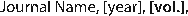
\includegraphics{head_foot/RF}}
\fancyfoot[CE]{\vspace{-7.2pt}\hspace{-14.2cm}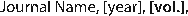
\includegraphics{head_foot/RF}}
\fancyfoot[RO]{\footnotesize{\sffamily{1--\pageref{LastPage} ~\textbar  \hspace{2pt}\thepage}}}
\fancyfoot[LE]{\footnotesize{\sffamily{\thepage~\textbar\hspace{3.45cm} 1--\pageref{LastPage}}}}
\fancyhead{}
\renewcommand{\headrulewidth}{0pt}
\renewcommand{\footrulewidth}{0pt}
\setlength{\arrayrulewidth}{1pt}
\setlength{\columnsep}{6.5mm}
\setlength\bibsep{1pt}
%%%END OF FOOTER%%%

%%%FIGURE SETUP - please do not change any commands within this section%%%
\makeatletter
\newlength{\figrulesep}
\setlength{\figrulesep}{0.5\textfloatsep}

\newcommand{\topfigrule}{\vspace*{-1pt}%
\noindent{\color{cream}\rule[-\figrulesep]{\columnwidth}{1.5pt}} }

\newcommand{\botfigrule}{\vspace*{-2pt}%
\noindent{\color{cream}\rule[\figrulesep]{\columnwidth}{1.5pt}} }

\newcommand{\dblfigrule}{\vspace*{-1pt}%
\noindent{\color{cream}\rule[-\figrulesep]{\textwidth}{1.5pt}} }

\makeatother
%%%END OF FIGURE SETUP%%%

%%%TITLE, AUTHORS AND ABSTRACT%%%
\twocolumn[
  \begin{@twocolumnfalse}
\vspace{3cm}
\sffamily
\begin{tabular}{m{4.5cm} p{13.5cm} }


\includegraphics{head_foot/DOI} & \noindent\LARGE{\textbf{Local Structure and Lithium Ion Diffusion Pathway of Cubic Li$_7$La$_3$Zr$_2$O$_{12}$ Studied by Total Scattering and the Reverse Monte Carlo Method$^\dag$}} \\%Article title goes here instead of the text "This is the title"
\vspace{0.3cm} & \vspace{0.3cm} \\

 & \noindent\large{Haolai Tian,$^{\ast,a}$}
 Xiang Yang Kong,$^{b}$
 Guanqun Cai,$^{c}$
 Lei Tan,$^{c}$
 Anthony E Phillip,$^{c}$
 Isaac Abrahams,$^{d}$
 David A Keen,$^{e}$
 Dean Keeble,$^{f}$
and Martin T. Dove,\textit{$^{g,h,\ddag}$}
\\%Author names go here instead of "Full name", etc.

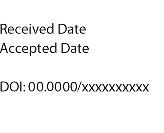
\includegraphics{head_foot/dates} & \noindent\normalsize{
The lithium-bearing oxide Li$_7$La$_3$Zr$_2$O$_{12}$ (LLZO), with the cubic garnet crystal structure, is an excellent candidate for solid electrolytes with its structural stability and high Li$^+$ conductivity. Here we use neutron and x-ray total scattering methods with the Reverse Monte Carlo method to identify the temperature-dependence of the Li$^+$ distribution and of the stability and flexibility of the basic oxide structure. We compare with the results with the outcomes from supporting molecular dynamics simulations. The results give insight into the mechanism  of Li$^+$ conductivity.
} \\

\end{tabular}

 \end{@twocolumnfalse} \vspace{0.6cm}

  ]
%%%END OF TITLE, AUTHORS AND ABSTRACT%%%

%%%FONT SETUP - please do not change any commands within this section
\renewcommand*\rmdefault{bch}\normalfont\upshape
\rmfamily
\section*{}
\vspace{-1cm}


%%%FOOTNOTES%%%

\footnotetext{\textit{$^{a}$~China Spallation Neutron Source (CSNS), Institute of High Energy Physics (IHEP), Chinese Academy of Sciences (CAS), Dongguan 523803, People's Republic of China}}
\footnotetext{\textit{$^{b}$~School of Materials Sciences and Engineering, Shanghai Jiao Tong University, Huashan Road 1954, Shanghai 200030, People's Republic of China}}
\footnotetext{\textit{$^{c}$~School of Physics and Astronomy, Queen Mary University of London, Mile End Road, London, E1 4NS, United Kingdom}}
\footnotetext{\textit{$^{d}$~School of Biological and Chemical Sciences, Queen Mary University of London, Mile End Road, London, E1 4NS, United Kingdom}}
\footnotetext{\textit{$^{e}$~ISIS Neutron and Muon Facility,  Rutherford Appleton Laboratory, Harwell Campus, Didcot, Oxfordshire, OX11 0QX, United Kingdom}}
\footnotetext{\textit{$^{f}$~Diamond Light Source Ltd, Harwell Science and Innovation Campus, Didcot, OX11 0DE, United Kingdom}}
\footnotetext{\textit{$^{g}$~College of computer science, Sichuan University, Chengdu, 610065, People's Republic of China}}
\footnotetext{\textit{$^{h}$~School of Physics, School of Sciences, Wuhan University of Technology, Wuhan, Hubei 430070, People's Republic of China}}
\footnotetext{\textit{$^{\ddag}$~Corresponding author. email: martin.dove@icloud.com}}


%%Please use \dag to cite the ESI in the main text of the article.
%%If you article does not have ESI please remove the the \dag symbol from the title and the footnotetext below.
%\footnotetext{\dag~Electronic Supplementary Information (ESI) available: [details of any supplementary information available should be included here]. See DOI: 00.0000/00000000.}
%%additional addresses can be cited as above using the lower-case letters, c, d, e... If all authors are from the same address, no letter is required

%\footnotetext{\ddag~Additional footnotes to the title and authors can be included \textit{e.g.}\ `Present address:' or `These authors contributed equally to this work' as above using the symbols: \ddag, \textsection, and \P. Please place the appropriate symbol next to the author's name and include a \texttt{\textbackslash footnotetext} entry in the the correct place in the list.}


%%%END OF FOOTNOTES%%%

%%%MAIN TEXT%%%%
\section{Introduction}

Lithium ion batteries have wide application on electric vehicles, mobile devices, and battery
farms for renewable energy storage.  However the commonly used liquid-based electrolytes have
disadvantages such as flammability, volatile  and operating temperature limitations.
Although all-solid-state lithium ion batteries (SSLBs) which are expected to enhance the safety
reliability and performance issues have been long sought, the conductivity of solid electrolytes can not
keep competing at the level of the existed liquid-based counterpart.

Most solid electrolytes require both high Li$^+$ conductivity and negligible electronic
conductivity. However, in many materials the requirement to match high ionic conductivity with high electrochemical stability for commercialised battery applications is problematic. Recently the lithium-containing oxide  Li$_7$La$_3$Zr$_2$O$_{12}$ (LLZO)\cite{Murugan:2007eg, Samson:2019eo, Kataoka:2020bg}, which crystallises with the cubic garnet structure, has attracted much attention as a potential solid electrolyte because it has both high Li$^+$ conductivity and is stabile against chemical
reaction with Li metal, moisture, air, as well as being able to support both low and high electrical potential differences.

LLZO actually exists in two phases \cite{Geiger:2011cg}, of
cubic and tetragonal symmetry, and the two phases show different Li$^+$ conductivities. The conductivity of the cubic
phase is two orders of magnitude higher than tetragonal one, $~3\times 10^{-4}$ S/cm \cite{Murugan:2007eg}
and $~1.63\times 10^{-6}$ S/cm \cite{Awaka:2009jv}, respectively.
This difference may be related to the distances between Li sites, disorder degree of Li atom, and isotropic diffusion pathways in the cubic phase.

A cubic garnet structure can be described \cite{Cussen:2011dg} as having a general chemical formula of the form A$_3$B$_2$(TO$_4$)$_3$, where the T site has tetrahedral coordination with oxygen (24 sites in the cubic unit cell), the B site has octahedral coordination (16 sites in the unit cell), and the larger A site has 8-fold coordination (24 sites in the unit cell). In LLZO the Zr$^{4+}$ cations are in the B sites, and the La$^{3+}$ cations are in the A site. The tetrahedral sites are occupied by Li$^+$ cations, but full occupancy would only accommodate 3 of the 7 cations of the chemical formula. In crystal structure refinements, sites of general symmetry and irregular coordination with oxygen atoms are associated with the positions of the remaining Li$^+$ cations. However, there are 96 of these sites, and therefore there must only be partial occupancy in this model. Indeed, with more than one position available to the Li$^+$ cations there is no reason why the the tetrahedral sites should be fully occupied, and this partial occupancy is what allows for three-dimensional ionic conductivity.

The atomic structure of LLZO has been studied by two complementary methods. The first is standard crystallography, with both x-ray \cite{Awaka:2009jv,Buschmann:2011jo,Geiger:2011cg, Awaka:2011il, DanielRettenwander:2016ei,Wagner:2016bh,Kataoka:2019go} and neutron \cite{Awaka:2009jv,Buschmann:2011jo,Xie:2011gv,Han:2012is,Li:2012fz,DanielRettenwander:2016ei,Wang:2014ic} beams, from which Li$^+$ sites can be identified and their site occupancies refined. Using a maximum entropy method it was possibly to visualise the Li$^+$ diffusion pathway \cite{Han:2012is}.
%Moreover, anisotropic atomic displacement parameters can shed some light on the possible diffusion mechanisms; in the refinements previously reported it is clear that the Li$^+$ cations on general positions show a distribution of positions that is strongly elongated along a possible diffusion pathway including the tetrahedral sites.
The second method is molecular dynamics simulation \cite{Wang:2014ic,Klenk:2015ey}, which has given results broadly consistent with the crystal structure refinements.

In this paper we use the methods of neutron and synchrotron x-ray total scattering methods together with the Reverse Monte Carlo (RMC) method to create an image of the Li$^+$ site disorder for a wide range of temperatures. The X-ray data are sensitive to the atomic numbers, which means that the data for  x-ray total scattering will be mostly sensitive to the La$^{3+}$ and Zr$^{4+}$ cations, and to a lesser extent to the O$^{2-}$ anions, but will have virtually no sensitivity to the Li$^+$ cations. On the other hand, neutron total scattering will have enhanced sensitivity to the O$^{2-}$ anions and, but to a lesser extent also, to the Li$^+$ cations. The combination of the two techniques will give greater chance to identify the spatial distribution of the  Li$^+$ cations.


\section{Experimental methods}

\subsection{Synthesis}
The precursor materials used was anhydrous LiOH (Alfa Aesar 99.5\%, dried at 200~$^{\circ}$C overnight; 10 wt.\% excess was taken to compensate for the loss of lithium under annealing conditions), La$_2$O$_3$ (Alfa Aesar, treated at 950~$^{\circ}$C overnight), ZrO$_2$ (Alfa Aesar, 99.7\%). The reactants were mixed with a mortar and pestle before reacting them at 950~$^{\circ}$C for 12 hours. The resultant product was reground and pressed into pellets. The pellets were transferred to an alumina crucible and buried with mother powder, followed by sintering at 1140~$^{\circ}$C for 20 hours to form single-phase material. The resulting pellets were grounded into powder and stored in an argon-filled glovebox (<0.1 ppm O$_2$, <0.1 ppm H$_2$O) to prevent reaction with humidity.


\subsection{Neutron Powder Diffraction and Total Scattering}

Neutron powder diffraction and total scattering data were obtained at a number of temperatures on the GEM diffractometer \cite{Hannon:2005cy} at the
ISIS spallation neutron source, Rutherford Appleton Laboratory, UK. The LLZO sample was contained in a cylindrical thin-walled vanadium can of 8 mm diameter.
This was mounted in a standard vanadium-foil furnace for measurements at and above room temperature (at 293 K, 450 K, 600 K, 750 K,
900 K and 1100 K). Data were collected on six separate occasions, counting for between 5 and 6 hours per temperature.

Measurements were also performed on the empty instrument, the empty furnace, and an empty vanadium can within the furnace to account for experimental background scattering and sources of beam attenuation, and also of an 8 mm diameter vanadium rod for normalisation. The data were processed using the GudrunN software \cite{Soper:2012vs} to obtain the scattering data and pair distribution function as described below, with a maximum scattering vector of $Q_\mathrm{max}$ of 50 \AA$^{-1}$. Diffraction data were also corrected and reduced using the Mantid software \cite{Arnold:2014iy}. Rietveld refinement of the crystal structures was performed by GSAS software \cite{Larson:2004wv} with the EXPGUI interface \cite{gsasgui}.

\begin{figure}[t]
\begin{center}
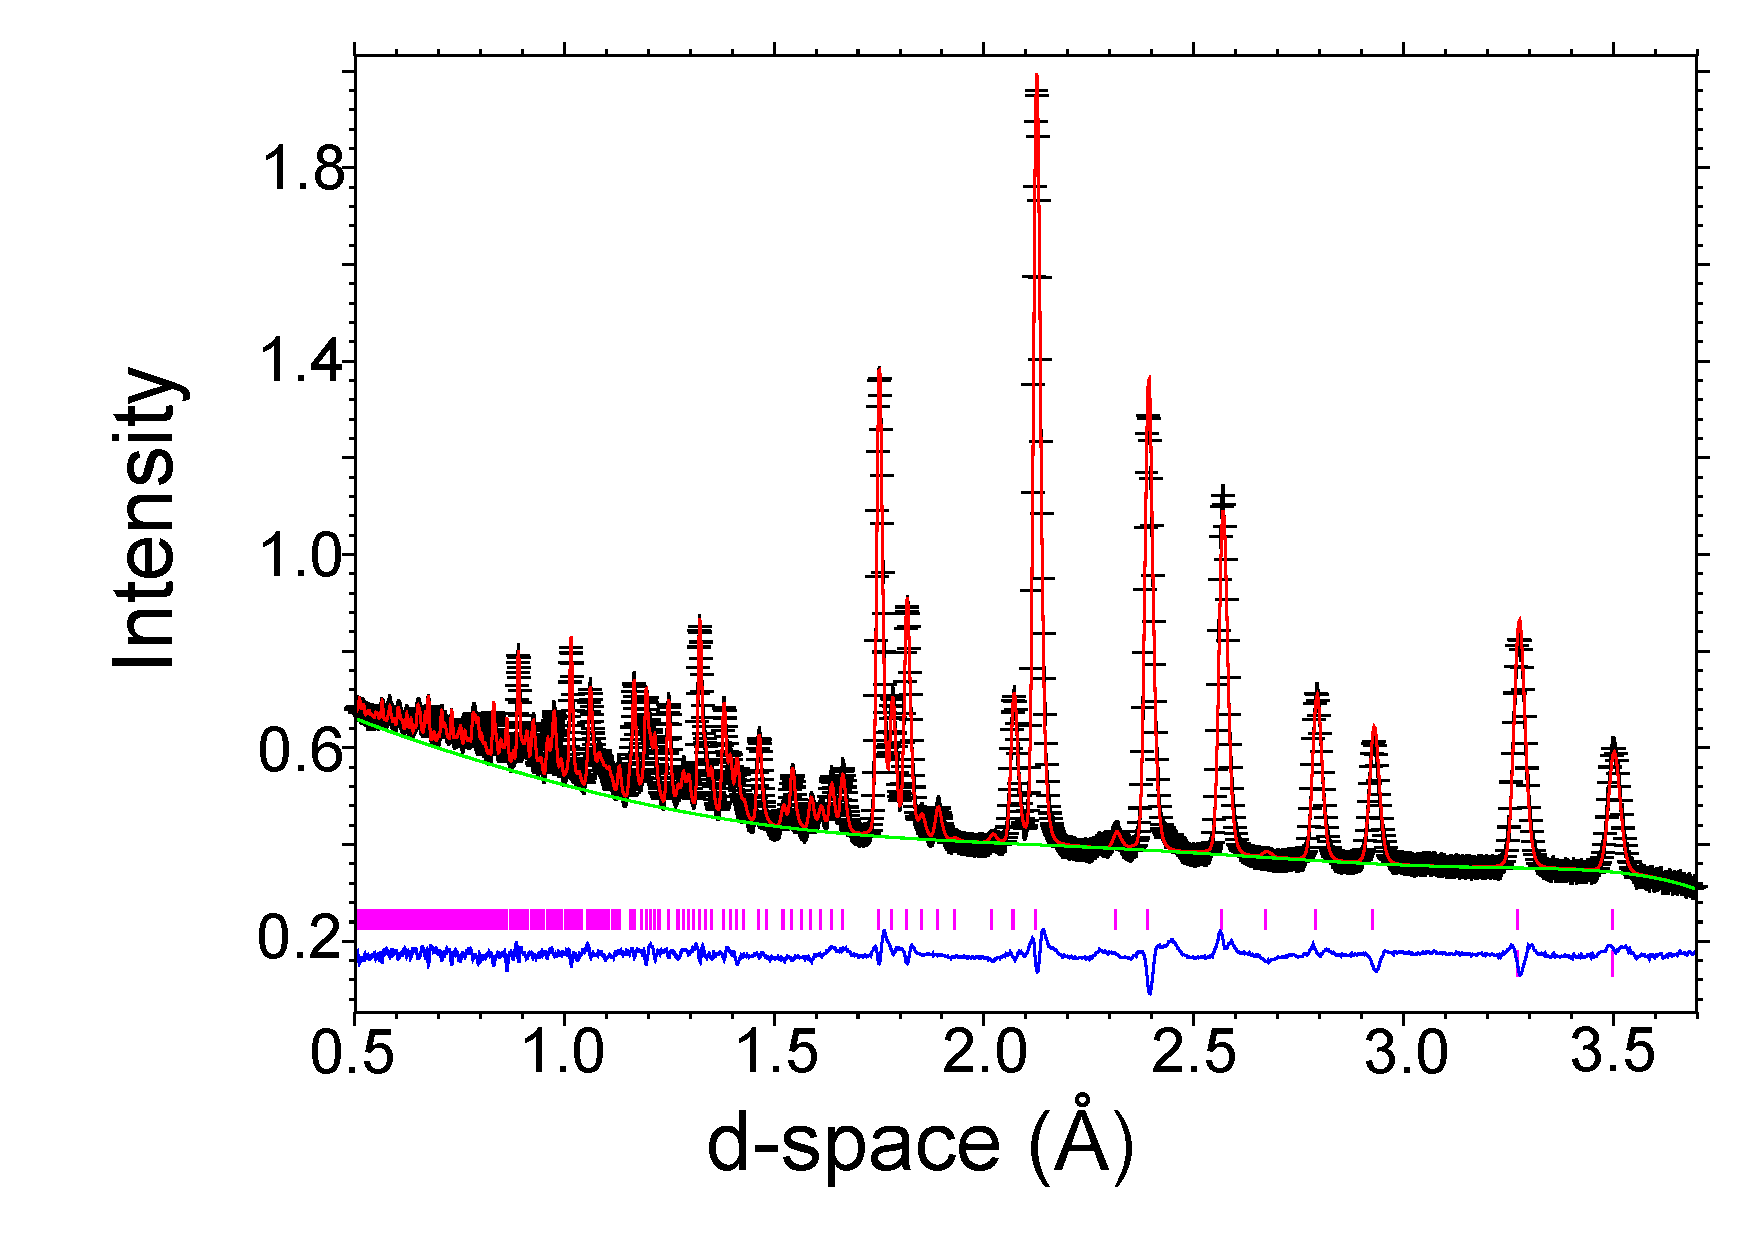
\includegraphics[width=0.4\textwidth]{Pics/1100KBank4v03.pdf}
\caption{Example of the quality of the Rietveld refinement of the crystal structure
 of LLZO from data collected from the $60^o$ (Bank 4) at temperature of 1100K.}
\label{fig:gsas}
\end{center}
\end{figure}


\subsection{Synchrotron  Total Scattering}
Synchrotron powder diffraction and total scattering data were collected on the XPDF beamline (I15-1 instrument) at Diamond Light Source (UK).
The X-rays were monochromatized to give a wavelength of 0.161669~\AA.
%PerkinElmer XRD 16611 CP3 and a PerkinElmer XRD 4343 CT were used as primary and secondary detectors.
The sample was sealed into borosilicate capillary tubes ($\phi$ 1 mm, and 50 mm in length) for measurements at the same temperatures as the neutron beam measurements. The raw data  were corrected and reduced into scattering data using the program DAWN \cite{Basham:2015cf}.
And PDF $D(r)$ were processed from scattering data using GudrunX \cite{Soper:2011fda,Soper:2012vs} with the range of data between $0.5 \le Q \le 25$ \AA$^{-1}$ for the Fourier transformation. Corrections for fluorescence were applied, in which the fluorescence energy of La was assumed to be 38.739 keV.

\begin{figure}[t]
\centering
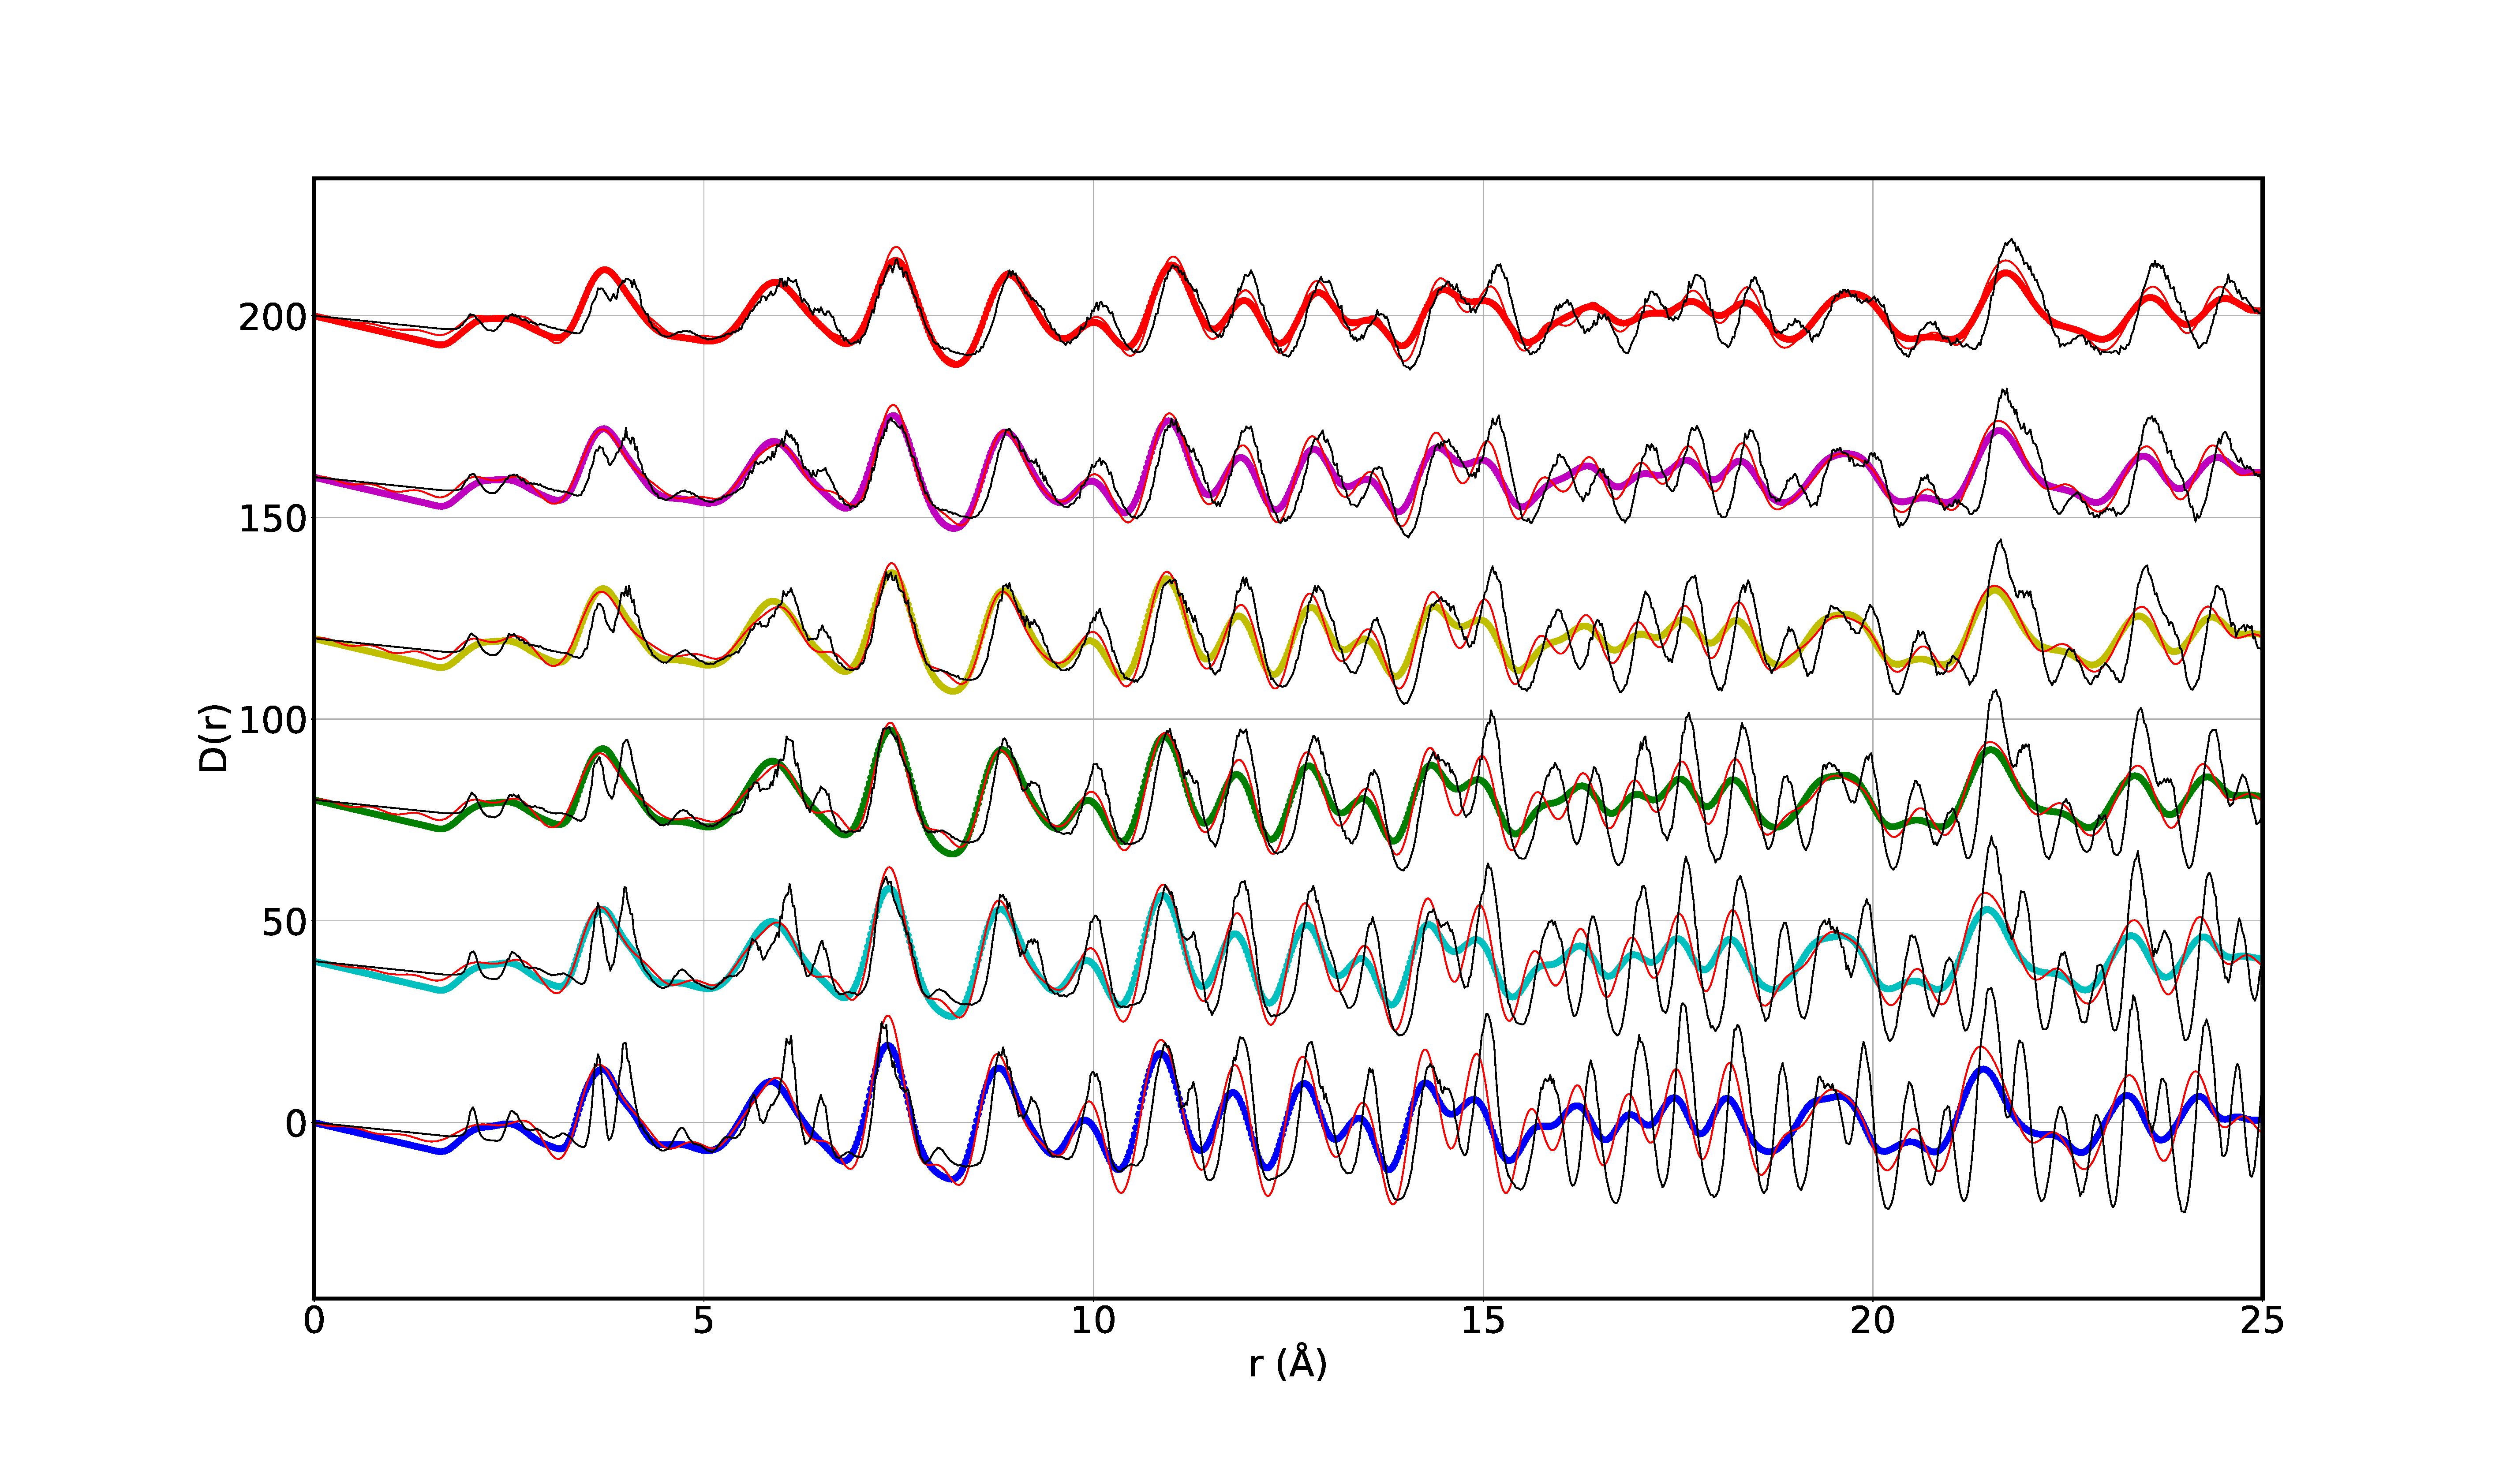
\includegraphics[width=0.5\textwidth]{Pics/xpdf.pdf}
\caption{Synchrotron pair distribution $D(r)$ obtained from GudrunX for all temperatures represented as circles.
 A constant offset has been applied to separate those curves.
 The solid black lines indicate the  simulated intensities from Dl\_poly, and RMC modelling are represented by the solid red lines.
 }
\label{fig:xpdf}
\end{figure}

\subsection{Pair Distribution Function}
The differential cross section for the scattering of a beam of radiation as integrated over all changes of energy is defined as
\begin{equation}
\frac{1}{N}\frac{d\sigma}{d\Omega}=I(Q)=I^\mathrm{S}(Q)+i(Q)
\end{equation}
where $I^\mathrm{S}(Q)=  \sum_m c_m f_m^2 $ is the self-scattering of all atoms, $c_m$ is the fractional amount of atom type $m$ such that $\sum_m c_m = 1$, and $f_m$ is the scattering factor of atom of type $m$ (the symbol $b_m$ is usually used for neutron scattering, denoting the scattering length whose value is independent of $Q$) \cite{Keen:2001wc}. The function $i(Q)$ is the total scattering structure factor. Here we define the partial pair distribution function (PDF) $g_{mn}(r)$ to represent the number of atoms of type $n$ within the shell between $r$ and  $r+\mathrm{d}r$ centred on a particle of type $m$, namely of value $4 \pi r^2 \mathrm{d}r \times c_n \rho \times g_{mn}(r)$,  where $\rho$ is the overall atomic number density. The structure factor $i(Q)$ can then be written as \cite{Dove2002}
\begin{equation}
i(Q)=4\pi\rho\int^{\infty}_{0}\sum_{m,n}c_m c_n f_m f_n r^2 [g_{mn}(r)-1]\frac{\sin{Qr}}{Qr} \mathrm{d}r
\end{equation}
 The overall pair distribution function is defined as
\begin{equation}\label{fun:dofr_0}
D(r)=4\pi\rho r \sum_{m,n}c_m c_n f_m f_n [g_{mn}(r)-1]
\end{equation}
so that
\begin{equation}
Qi(Q)=\int^{\infty}_{0} D(r) \sin{Qr} \mathrm{d}r
\end{equation}
In turn, the function $D(r)$ can be obtained as the the sine Fourier transform of $Qi(Q)$, but in practice the transform is modified as
\begin{equation}\label{fun:dofr_1}
D(r)=\frac{2}{\pi}\int^{Q_{max}}_{0} M(Q)Qi(Q)\sin{Qr} \mathrm{d}r
\end{equation}
where $M(Q) = \sin(\pi Q/Q_\mathrm{max})/(\pi Q/Q_\mathrm{max})$ is the Lorch function, which is introduced to reduce the effect of finite maximum momentum transfer, $Q_\mathrm{max}$ \cite{Lorch:1969js, Dove2002, Soper:2012kr}. Those tasks were carried out using the programs GudrunX and GudrunN \cite{Soper:2011fda,Soper:2012vs}.


\begin{figure}[t]
\centering
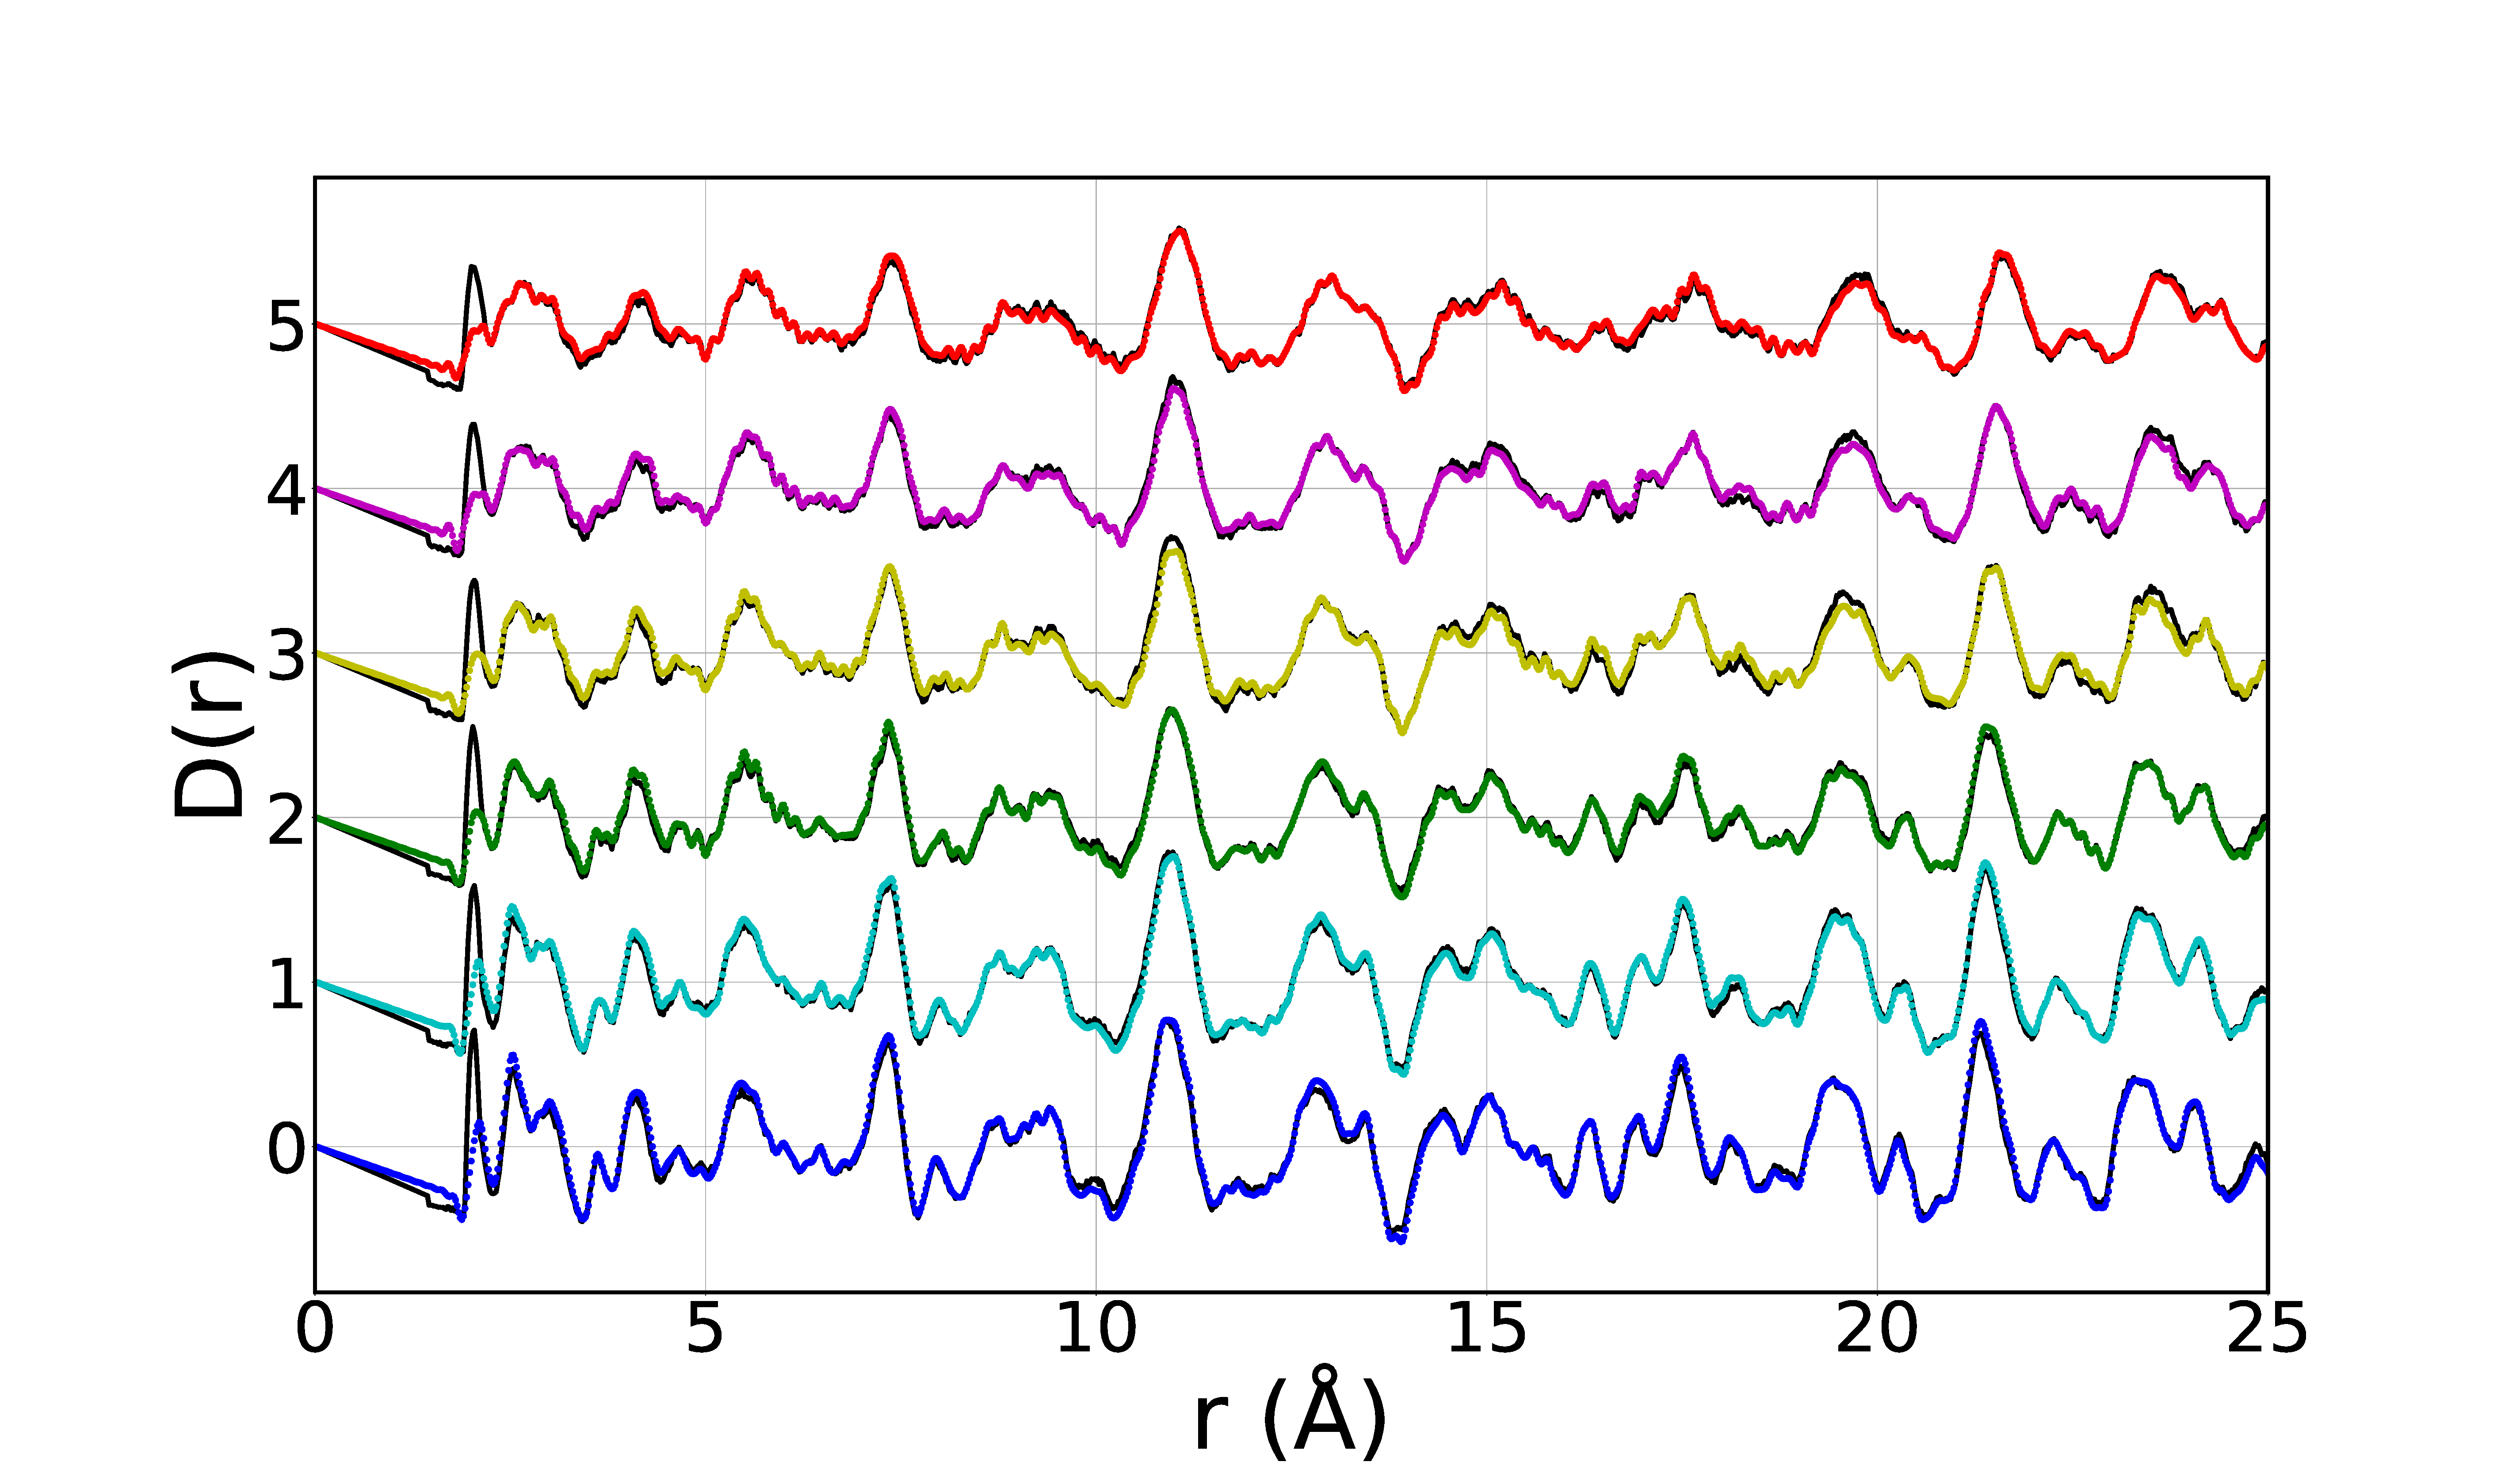
\includegraphics[width=0.5\textwidth]{Pics/npdf.pdf}
\caption{Neutron pair distribution $D(r)$  obtained from GudrunN for all temperatures represented as circles.
 A constant offset has been applied to separate those curves.
 The solid black lines indicate the  simulated intensities from Dl\_poly, and RMC modelling are represented by the solid red lines. }
\label{fig:npdf}
\end{figure}

\subsection{Reverse Monte Carlo Analysis}

The Reverse Monte Carlo (RMC) method, whilst initially developed for the study of highly-disordered (non-crystalline) materials \cite{McGreevy:1988bu}, is in fact an excellent technique for the study of disordered crystalline materials \cite{Keen:2005dd}. That said, it appears that there have been only limited applications of the RMC method to crystalline fast-ion conductors \cite{Adams:2000ez, Swenson:2001if, Adams:2002ga,Adams:2005ds}, and apparently not to the cases where lithium is the mobile ion. We will comment later on some observations on the application of the RMC method to lithium fast-ion conductors in the light of the experience gained in this study.

The RMC method is a way to visualise the atomic-scale structure of a material through a simulation based on experimental data. If uses a Monte Carlo method to minimise the difference between experimental functions and the values computed from the atomic configuration as expressed in the function
\begin{equation}
\chi^2=\sum_{j}\sum_{i}(y^ \mathrm{obs}_{i,j}-y^ \mathrm{calc}_{i,j})^2/\sigma^2_{j}
\end{equation}
where $y^\mathrm{obs}_{i,j}$ is the observed values at data point $i$ in data set $j$, $y^ \mathrm{calc}_{i,j}$ is the calculated counterpart, and  $\sigma^2_{j}$ is weighing function that may represent the statistical accuracy of data set. In this study, the data sets used include $i(Q)$ from both neutron and  synchrotron power diffraction, $D(r)$ from the neutron total scattering data, and the Bragg data from the neutron diffraction measurements, In the RMC method an selected at random is moved by a random amount up to a specified maximum. The move is accepted if the value of $\chi^2$ is lowered. On the other hand, if the value of $\chi^2$ increases by an amount $\Delta \chi^2$, the move is accepted only with probability $\exp(-\Delta \chi^2/2)$. Each simulation ran until the value of $\chi^2$ had reached a stable minimum value, corresponding in this case to around 300 accepted moves per atom.

The RMC simulations were performed using the program \texttt{RMCprofile} v6.7 \cite{Tucker:2007eh}. The starting configurations of Li$_7$La$_2$Zr$_3$O$_{12}$ were generated from the results of Rietveld refinement using the \texttt{data2config}/\texttt{RMCcreate} program \cite{Dove:2013gk}. Configurations were $4\times 4\times 4$ supercell of the conventional body-centred unit cell with linear dimension of around 52 \AA, containing 12288 atoms. Maximum atomic moves of La, O and Zr atoms were of size $0.05 \AA$, but those of Li were $0.1 \AA$. Minimum distance constraints were applied within the RMC simulation; between  pairs of atoms as given in Table  \ref{tab:min_dis}. Finally, bond-stretching and bond-bending potentials were applied within the ZrO$_6$ octahedra, and for the La--O bonds, during the RMC simulation.

\begin{figure}[t]
\centering
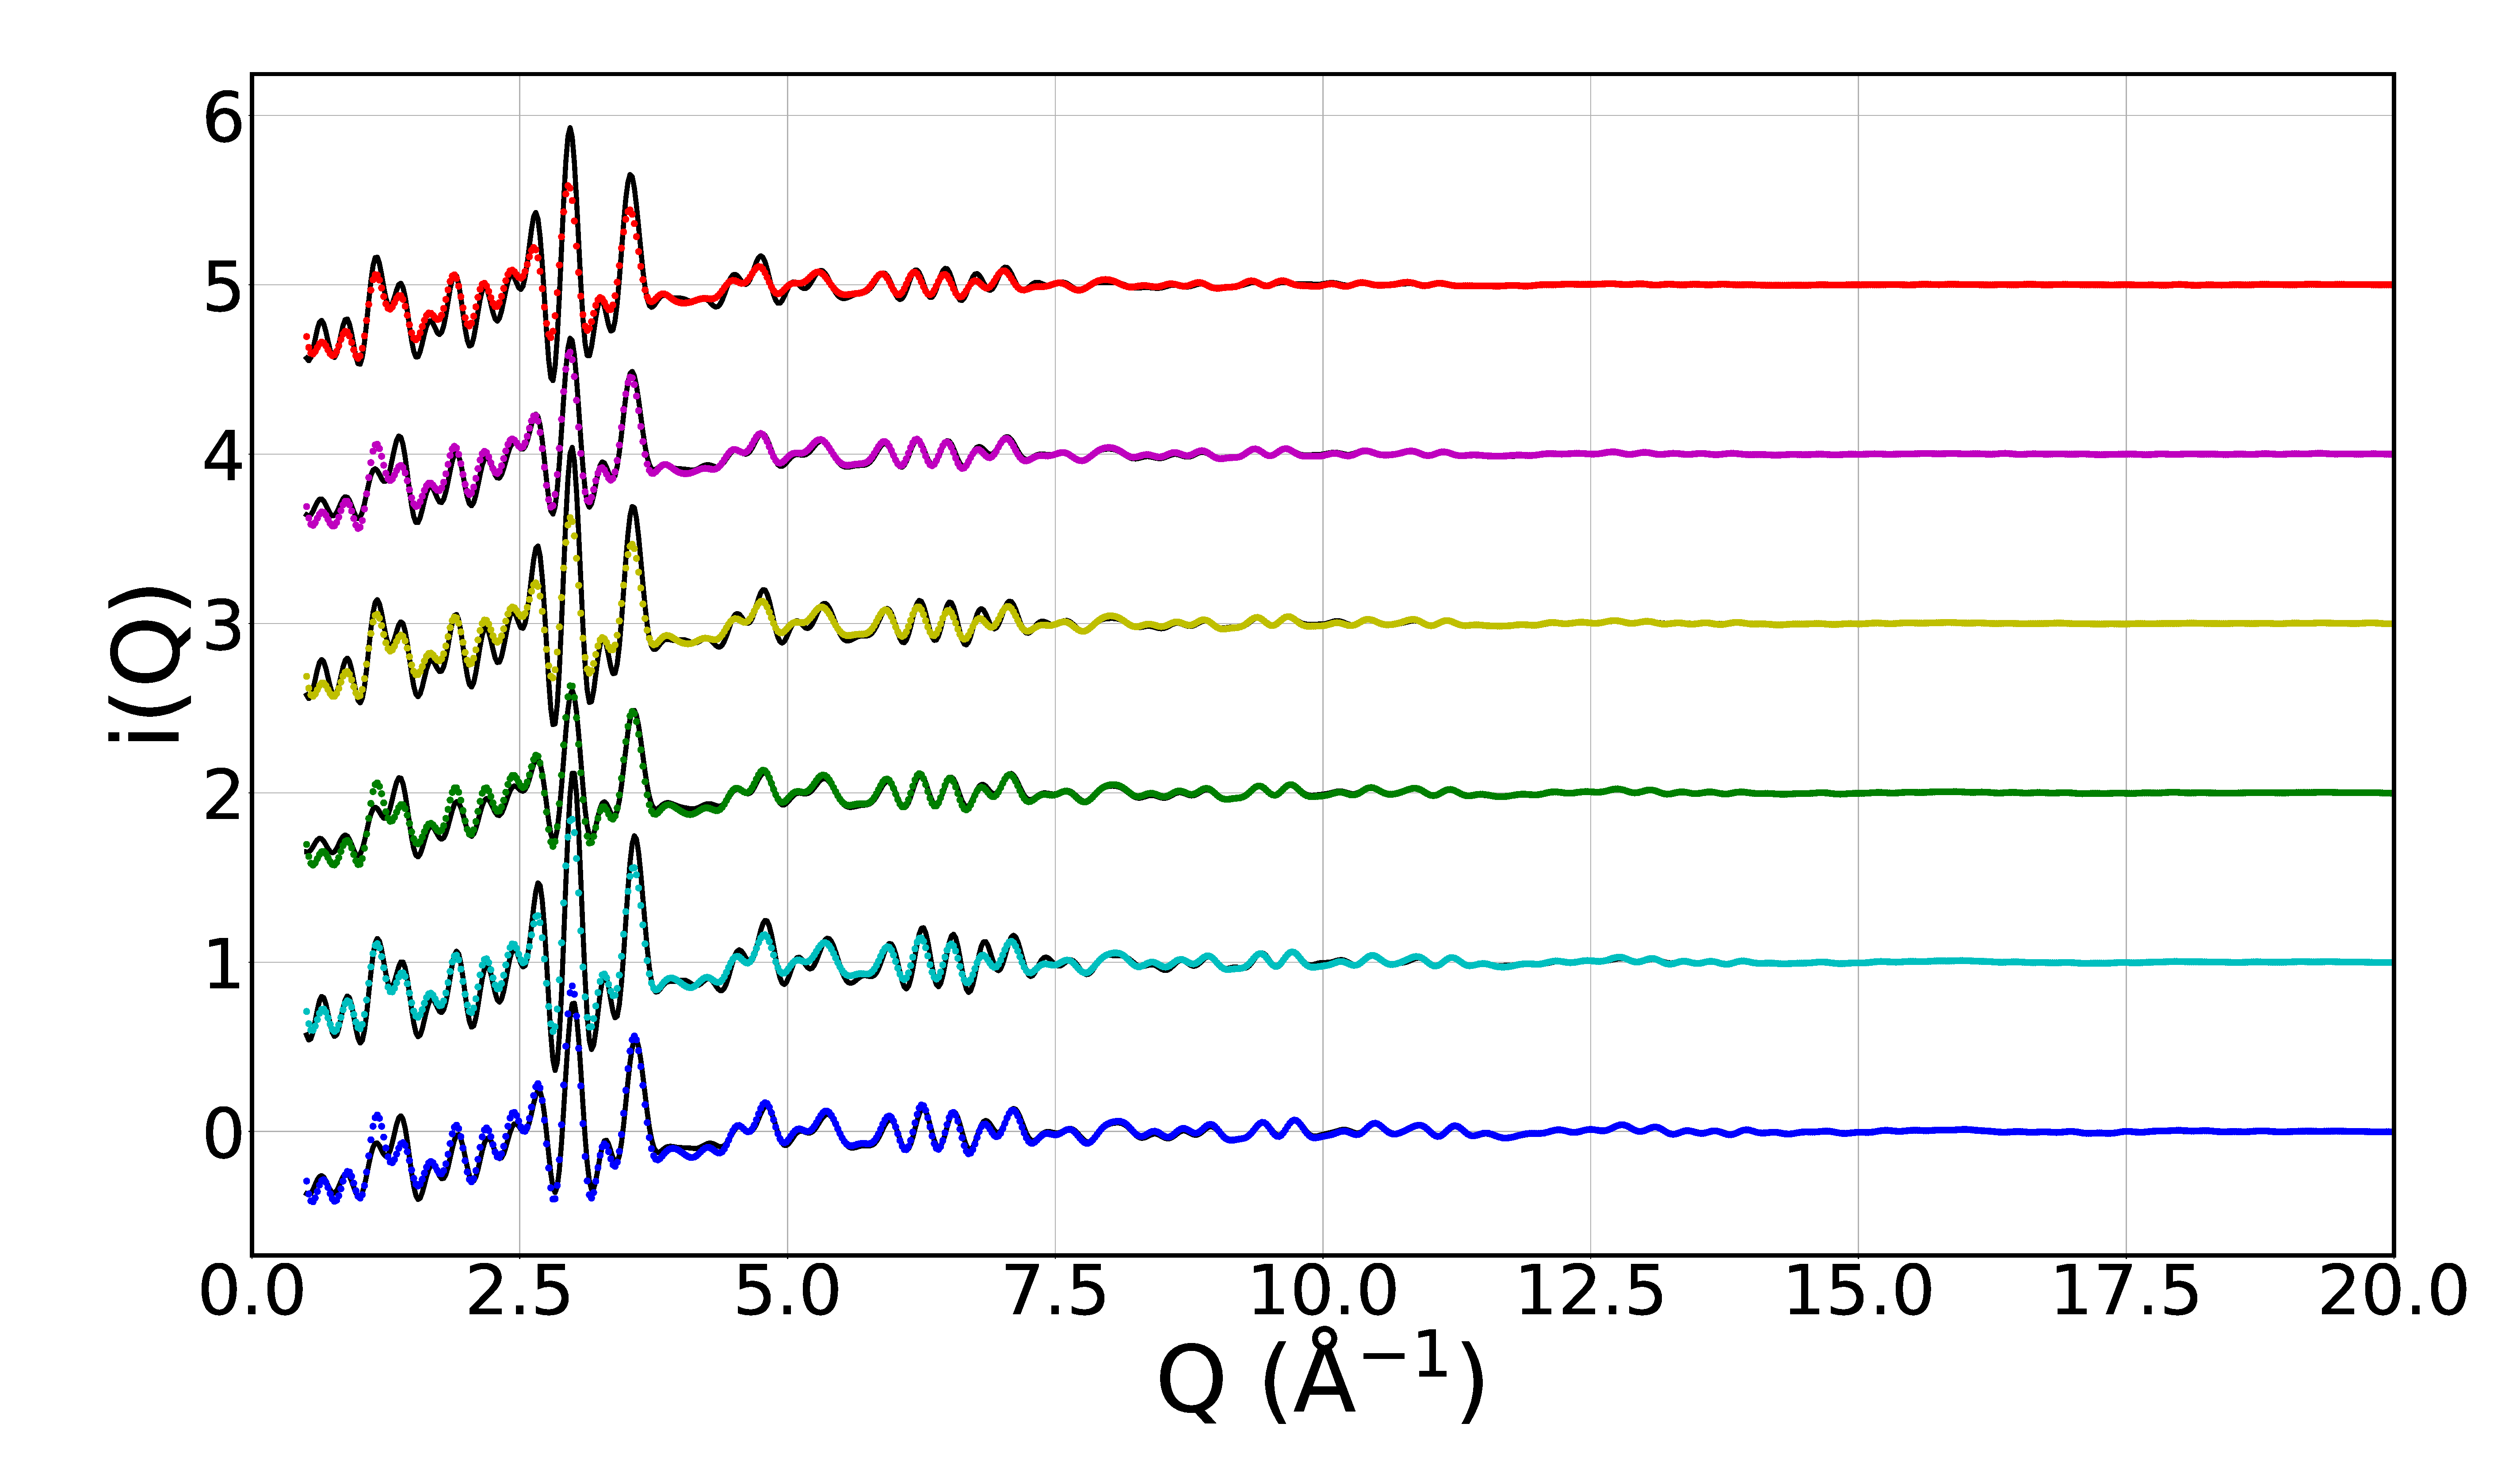
\includegraphics[width=0.5\textwidth]{Pics/nsoq.pdf}
\caption{Neutron scattering function $S(Q)$ for all temperatures. A constant offset has been applied to separate those curves.}
\label{fig:nsoq}
\end{figure}

\begin{table}[t]
\centering
\caption{The minimum distances between pairs of atoms} \label{tab:min_dis}
\begin{tabular}{c|cccc}
\hline
   & Li & O & Zr & La \\
\hline
Li & 1.69 & 1.50 & 2.3 & 2.3 \\
O  &      & 2.2  & 1.79& 2.2 \\
Zr &      &      & 5.0 & 3.3 \\
La &      &      &     & 3.3 \\
\hline
\end{tabular}
\end{table}

\subsection{Electrochemical Impedance Measurements}

Electrochemical experiments were carried out in an Ar glovebox (O$_2$; H$_2$O < 1 ppm). For the electrical measurement,
gold electrodes were evaporated on LLZO by thermal evaporation. The EIS was recorded by a Solartron ModuLab system,
and contacted via a probe station on a hot stage in the glovebox. EIS was performed with an 10 mV amplitude voltage
in a frequency range of 50 mHz to 1 MHz.


\subsection{Molecular Dynamic Simulation}

Classical molecular dynamics (MD) simulations were performed using the \texttt{DL\_POLY} package \cite{Todorov:2006ee}.
Empirical force-fields were used, which include the long-range Coulomb potential,
short-range Buckingham potential functions to describe the energy between two ions of type $m$ and $n$, $E_{mn}(r)$, assumed to be functions of inter-ionic separation $r$ only:
\begin{equation} \label{eq:buckingham}
E_{mn}(r) = \frac{Q_m Q_n}{4 \pi \epsilon_0 r} + A_{mn} \exp(-r/\rho_{mn}) - C_{mn}r^{-6}
\end{equation}
with ions treated as rigid entities with no induced polarisation, and assigned formal charges, $Q_\mathrm{Zr} = +4e$, $Q_\mathrm{La} = +4e$, $Q_\mathrm{Li} = +e$, $Q_\mathrm{O} = -2e$, where $e$ is the positive unit charge value. The parameters of the force-field were taken from the work of Wang et al  \cite{Wang:2014ic}, who used a combination of literature and new values; the parameters of the force field are given in Table \ref{tab:md_force}. The starting configurations were the same as used in the RMC work (linear dimensions of around 52 \AA, and 12288 atoms), and simulations were performed at the same temperatures as in the neutron and x-ray total scattering measurements.

Simulations were performed within thermodynamic ensembles that were either constant-stress \cite{Parrinello:1980kx, Melchionna:2006fi} and constant temperature \cite{Nose:1984bf, Hoover:1985cu}, or the standard constant-volume constant-energy microcanonical conditions. Simulations were performed using a time step of 0.001 ps, allowing 5 ps for equilibration.


%\begin{table}[h]
%\centering
%\caption{Force-field parameters} \label{tab:md_force}
%\begin{tabular}{cccccc}
%\hline
%      & \multicolumn{3}{c}{Buckingham parameters}    & \multicolumn{2}{c}{O shell parameters}         \\
%\hline
%      & A (eV)  & $\rho$(\AA) & C(eV\AA$^6$)         &                    &       \\
%Zr-O  & 1385.02 & 1.79        & 0                    & Y (e)              &  -2.76\\
%La-O  & 4579.23 & 0.3044      & 0                    & k (eV $\AA^{-2}$)  &  30.2 \\
%Li-O  & 632.102 & 0.2906      & 0                    & m (au)             &  0.2  \\
%O-O   & 22764.30& 0.1490      & 27.63                &                    &       \\
%\hline
%\end{tabular}
%\end{table}

\begin{table}[t]
\centering
\caption{Force-field parameters for the molecular dynamics simulations, from the work of Wang et al \cite{Wang:2014ic}, with interactions between cations assumed to be give only by the Coulomb interaction. Ions are assigned their formal charge values. The parameters are defined by equation \ref{eq:buckingham}.} \label{tab:md_force}
\begin{tabular}{cccccc}
\hline
      & $A$ (eV)  & $\rho$ (\AA) & $C$ (eV\,\AA$^6$)           \\
\hline
Zr--O  & 1385.02 & 1.79        & 0                      \\
La--O  & 4579.23 & 0.3044      & 0                      \\
Li--O  & 632.102 & 0.2906      & 0                      \\
O--O   & 22764.30& 0.1490      & 27.63                  \\
\hline
\end{tabular}
\end{table}

\begin{figure}[t]
\centering
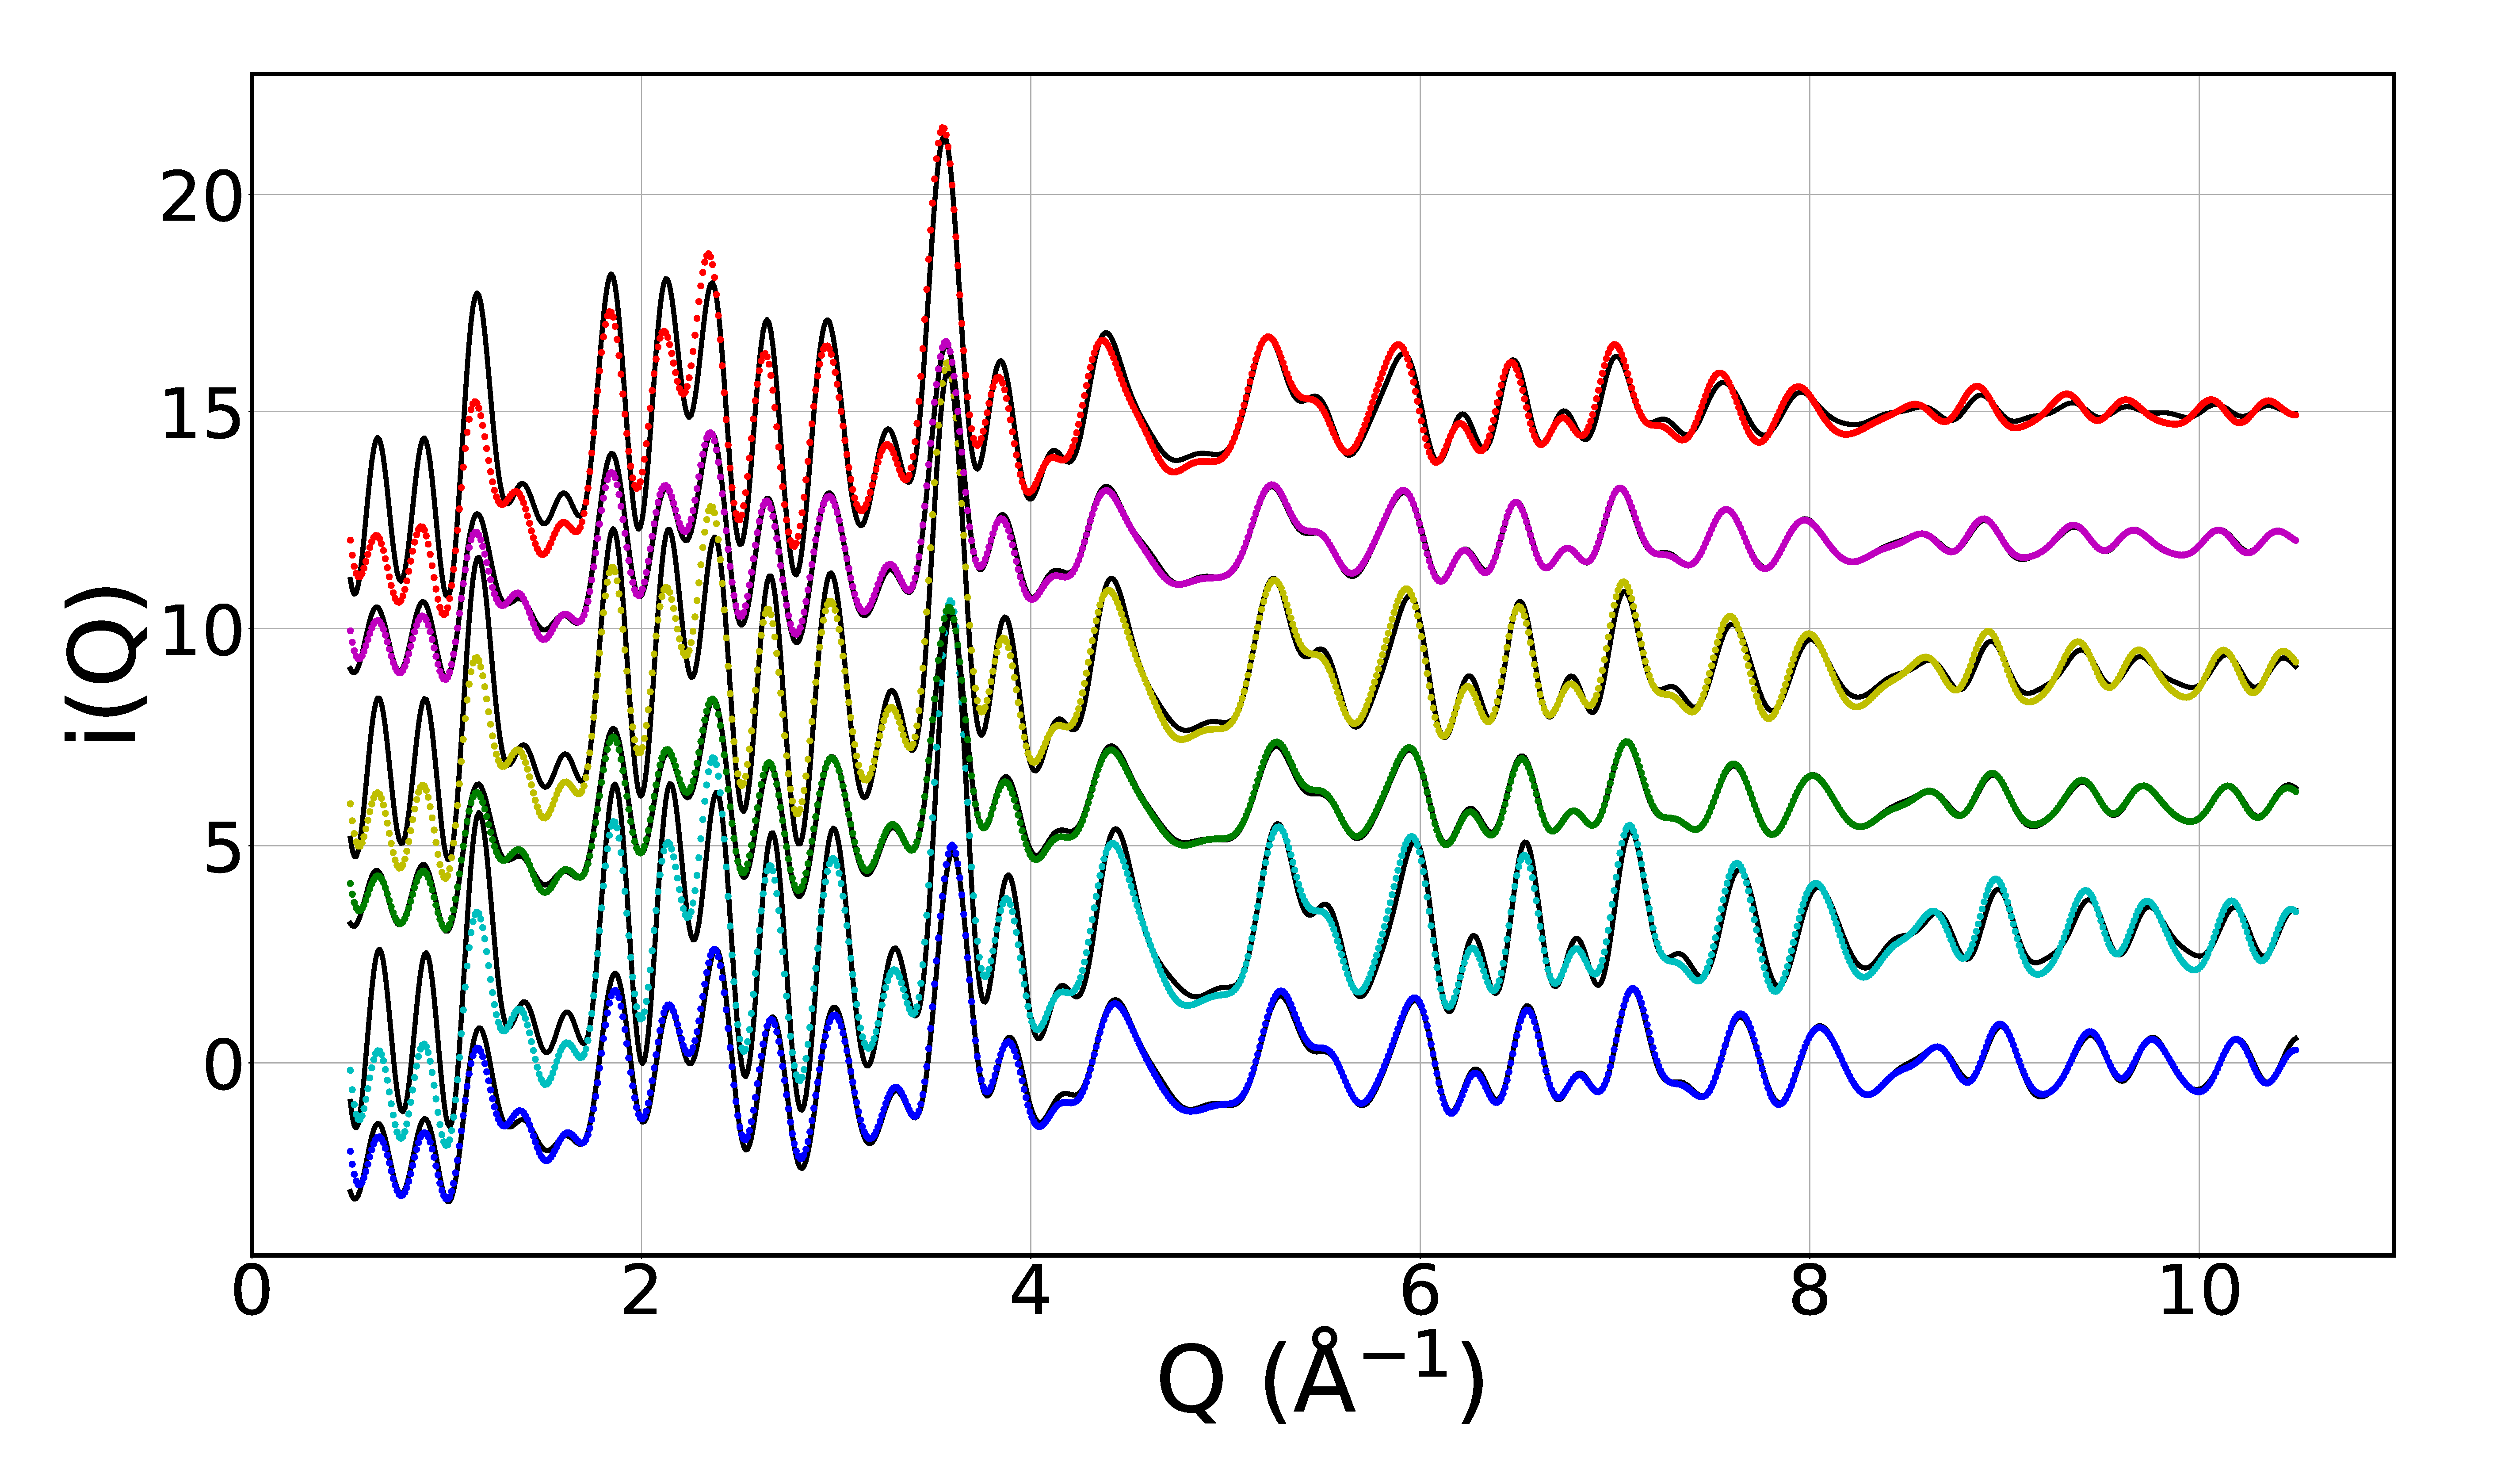
\includegraphics[width=0.5\textwidth]{Pics/xsoq.pdf}
\caption{Synchrotron scattering function $S(Q)$ for all temperatures. A constant offset has been applied to separate those curves.}
\label{fig:xsoq}
\end{figure}




%\subsection{GASP analysis}
%
%Both our RMC and MD configurations have been analysed using the GASP method.
%In this method the motions of the atoms associated with each polyhedron in
%the configuration are described together as a combination of whole-polyhedron rotation,
%bond-bending and bond-stretching motions.


\section{Results and discussion}

\subsection{Crystal Structure Analysis}

The structural parameters of Rietveld refinement for all temperatures are listed in Table \ref{tab:Rietveld_structure} and \ref{tab:Li_displacement_parameters},
which fitted well to the cubic model with space group $Ia\bar{3}d$. A sample fit to the data, namely for the data at 1100 K, is shown in Fig. \ref{fig:gsas}
The lattice parameters are plotted as functions of temperature in Fig. \ref{fig:lattice}, showing a linear thermal expansion. The coefficient of volumetric thermal expansion is $\alpha_V = 1.18 \times 10^{-5}$ K$^{-1}$. The structure is in good agreement with previous structure refinements \cite{Awaka:2009jv,Buschmann:2011jo,Geiger:2011cg, Awaka:2011il, DanielRettenwander:2016ei,Wagner:2016bh,Kataoka:2019go, Xie:2011gv,Han:2012is,Li:2012fz,Wang:2014ic}; aspects of the crystal structure have been discussed in these previous works.


\begin{table*}[t]
\centering
\caption{Lattice parameters, atomic fractional coordinates and Lithium site occupancy of Li$_7$La$_2$Zr$_3$O$_{12}$ obtained from Rietveld refinement. Zr has fractional coordinates 0,0,0, La has fractional coordinates $1/4,0,1/4$, Li$_1$ has fractional coordinates $3/8,0,1/4$, and Li$_2$ has fractional coordinates $1/4,y,z$. Standard deviations are given for the last significant figures in brackets. }
\label{tab:Rietveld_structure}
\begin{tabular}{ccccccccc}
\hline
\hline
$T$ (K)  & $a$ (\AA) & O ($x$)        & O ($y$)        & O ($z$)        &  Li$_2$ ($y$)       & Li$_2$ ($z$) & Li$_2$ ($occ.$) \\
\hline
273  & 12.9219(1)    & 0.1021(1)      & 0.1970(1)      & 0.28162(9)     & 0.1763(5)           & 0.4263(5)    & 0.507(4) \\
450  & 12.95247(9)   & 0.10210(8)     & 0.19666(8)     & 0.28141(7)     & 0.1761(2)           & 0.4261(2)    & 0.524(3) \\
600  & 12.97967(9)   & 0.10210(8)     & 0.19717(8)     & 0.28136(7)     & 0.1774(3)           & 0.4274(3)    & 0.524(4) \\
750  & 13.0096(2)    & 0.1019(1)      & 0.19686(9)     & 0.28123(8)     & 0.1754(4)           & 0.4254(4)    & 0.537(4) \\
900  & 13.04123(9)   & 0.10235(8)     & 0.19751(8)     & 0.28060(7)     & 0.1766(3)           & 0.4266(3)    & 0.540(3) \\
1100 & 13.08634(8)   & 0.10184(7)     & 0.19742(6)     & 0.28081(6)     & 0.1772(2)           & 0.4272(2)    & 0.504(4) \\
\hline
\hline
\end{tabular}
\end{table*}

\begin{table*}[t]
\centering
\caption{Li displacement parameters $100 \times U_{ij}$(\AA$^2$) refined from Rietveld refinement.For Li$_2$ $U_{22} = U_{33}$ and $U_{12} = - U_{13}.
$. $U_{ij}$ units are in \AA$^2$.
Standard deviations are given for the last significant figures in brackets. }
\label{tab:Li_displacement_parameters}
\begin{tabular}{ccccccccc}
\hline
\hline
$T$ (K) & Li$_1$ $U_\mathrm{iso}$  & Li$_2$ $U_{11}$ & Li$_2$ $U_{22}$ & Li$_2$ $U_{12}$ & Li$_2$ $U_{23}$  & O $U_\mathrm{iso}$  & La $U_\mathrm{iso}$  & Zr $U_\mathrm{iso}$\\
\hline
273     &  0.9(5)                  & 10(1)           & 0.09(33)        & -3.6(5)         & -1.4(3)          &  0.97(2)            &  0.63(2)             &  0.62(3)            \\
450     & -0.6(2)                  & 13(1)           & 0.2(2)          & -6.1(4)         & -2.5(2)          &  0.97(1)            &  0.56(2)             &  0.35(2)            \\
600     &  1.4(8)                  & 14(1)           & 0.5(2)          & -4.4(4)         & -2.3(3)          &  1.7(1)             &  1.16(2)             &  1.03(3)            \\
750     & -2.8(2)                  & 19(1)           & 1.9(5)          & -10.7(8)        & -4.9(5)          & -0.20(1)            & -0.01(2)             & -0.43(2)            \\
900     & -2.7(1)                  & 16(1)           & 0.4(3)          & -7.4(5)         & -3.1(3)          &  0.74(1)            &  0.38(2)             & -0.10(2)            \\
1100    &  3.7(7)                  & 16(1)           &-0.6(2)          & -5.4(4)         & -2.9(2)          &  1.97(1)            &  1.39(2)             &  0.93(2)            \\
\hline
\hline
\end{tabular}
\end{table*}


%\begin{table*}[t]
%\centering
%\caption{Atomic (Except Li) displacement parameters $100 \times U_{ij}$ (\AA$^2$) refined from Rietveld refinement.
%$U_{ij}$ units are in \AA$^2$.
%Standard deviations are given for the last significant figures in brackets.  }
%\label{tab:atomic_parameters}
%\begin{tabular}{ccccccccc}
%\hline
%\hline
%T(K)   & O $U_{11}$ & O $U_{22}$ & O $U_{33}$ & O $U_{12}$ & O $U_{13}$ & O $U_{23}$  & La $U_\mathrm{iso}$    & Zr $U_\mathrm{iso}$Li$_7$    \\
%\hline
%273    & 0.382(44)  & 1.017(52)  & 0.425(44)  & -0.303(39) & -0.052(36) & 0.261(38)   & 0.281(15)  & 0.240(22)  \\
%450    & 0.838(49)  & 1.266(57)  & 0.822(52)  & -0.056(45) & -0.005(42) & 0.177(43)   & 0.622(19)  & 0.599(27)  \\
%600    & 1.430(43)  & 2.357(52)  & 1.830(51)  & -0.124(40) &  0.096(39) & 0.309(41)   & 1.168(17)  & 1.117(23)  \\
%750    & 1.238(60)  & 2.437(75)  & 1.653(72)  & -0.448(56) &  0.189(55) & 0.471(58)   & 0.861(24)  & 0.636(30)  \\
%900    & 0.014(92)  & 1.25(12)   & 0.211(98)  & -0.536(85) & -0.090(76) & 0.414(86)   & 0.340(40)  & 0.083(50)  \\
%1100   & 1.199(73)  & 3.172(97)  & 1.941(88)  & -0.041(70) &  0.404(68) & 0.189(73)   & 0.724(28)  & 0.404(34)  \\
%\hline
%\hline
%\end{tabular}
%\end{table*}

\begin{figure}[t]
\centering
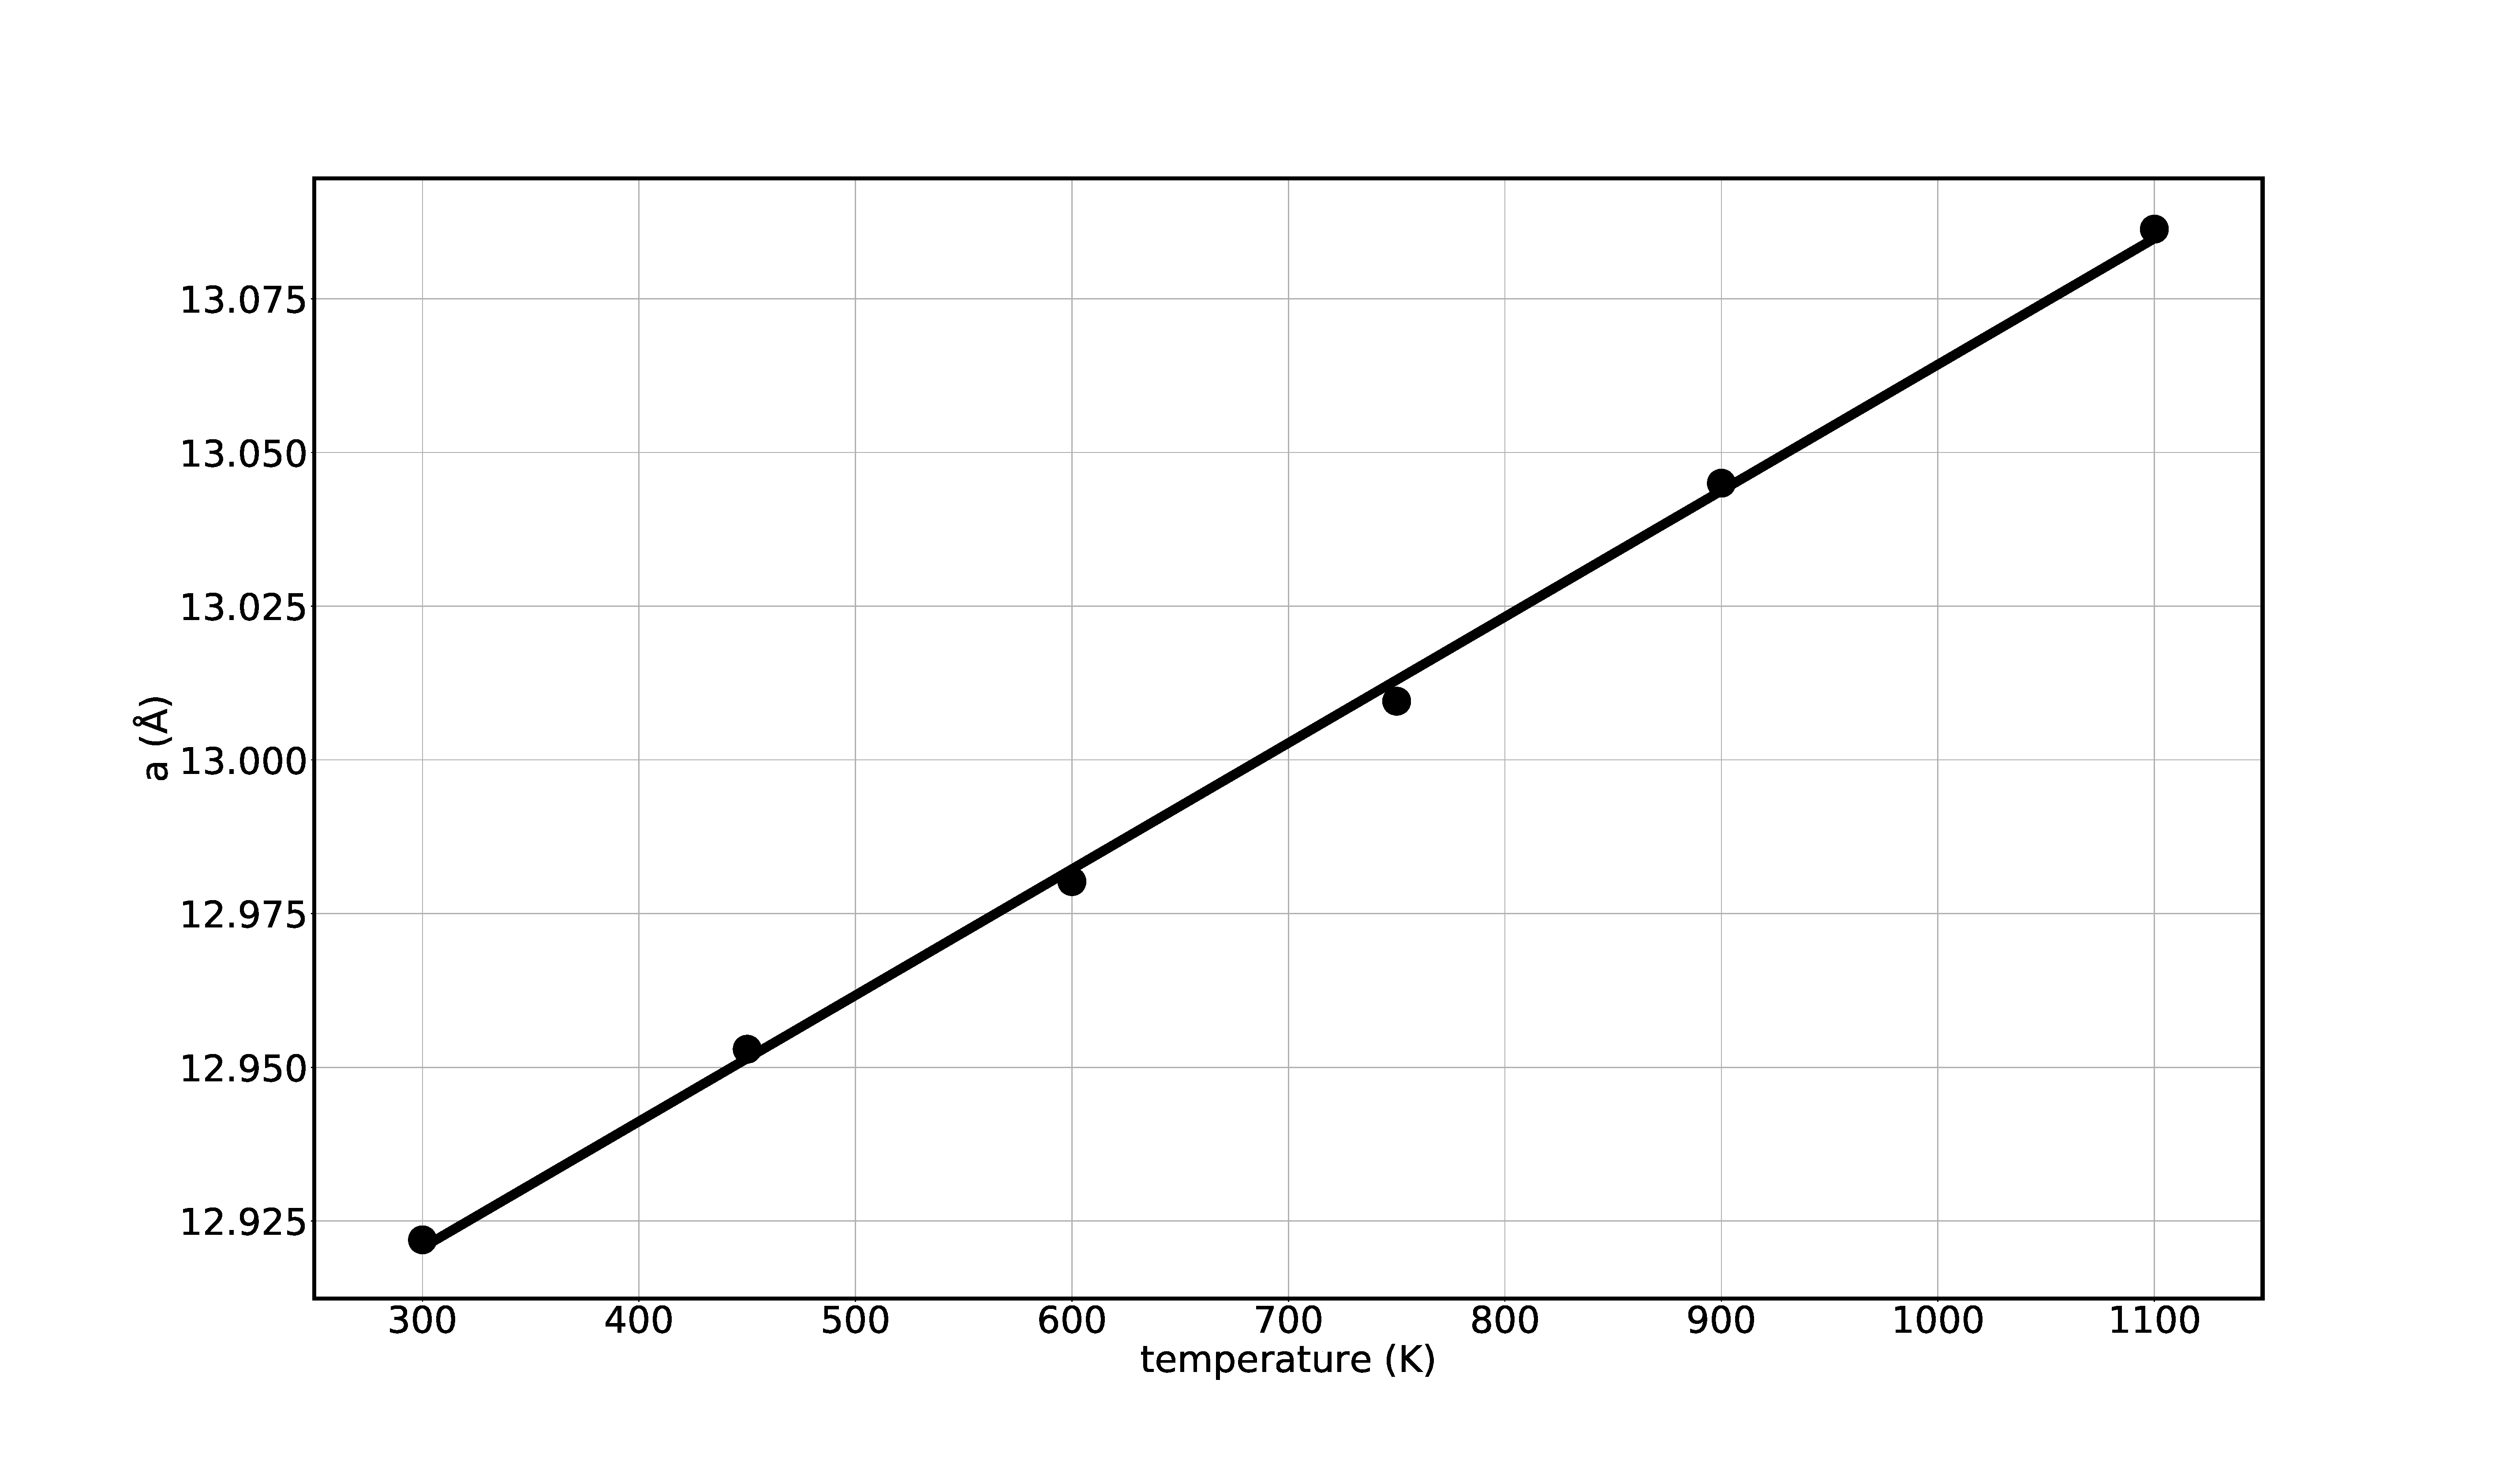
\includegraphics[width=0.5\textwidth]{Pics/lattice.pdf}
\caption{Variation of the lattice parameter of Li$_7$La$_2$Zr$_3$O$_{12}$ with temperature as obtained by Rietveld analysis (Table \ref{tab:Rietveld_structure}). }
\label{fig:lattice}
\end{figure}

%the average structure calculated from the RMC configurations agreed well with Rietveld refinement, as shown in Fig. \ref{fig:Rietveld_refinement}



\begin{figure}[t]
\centering
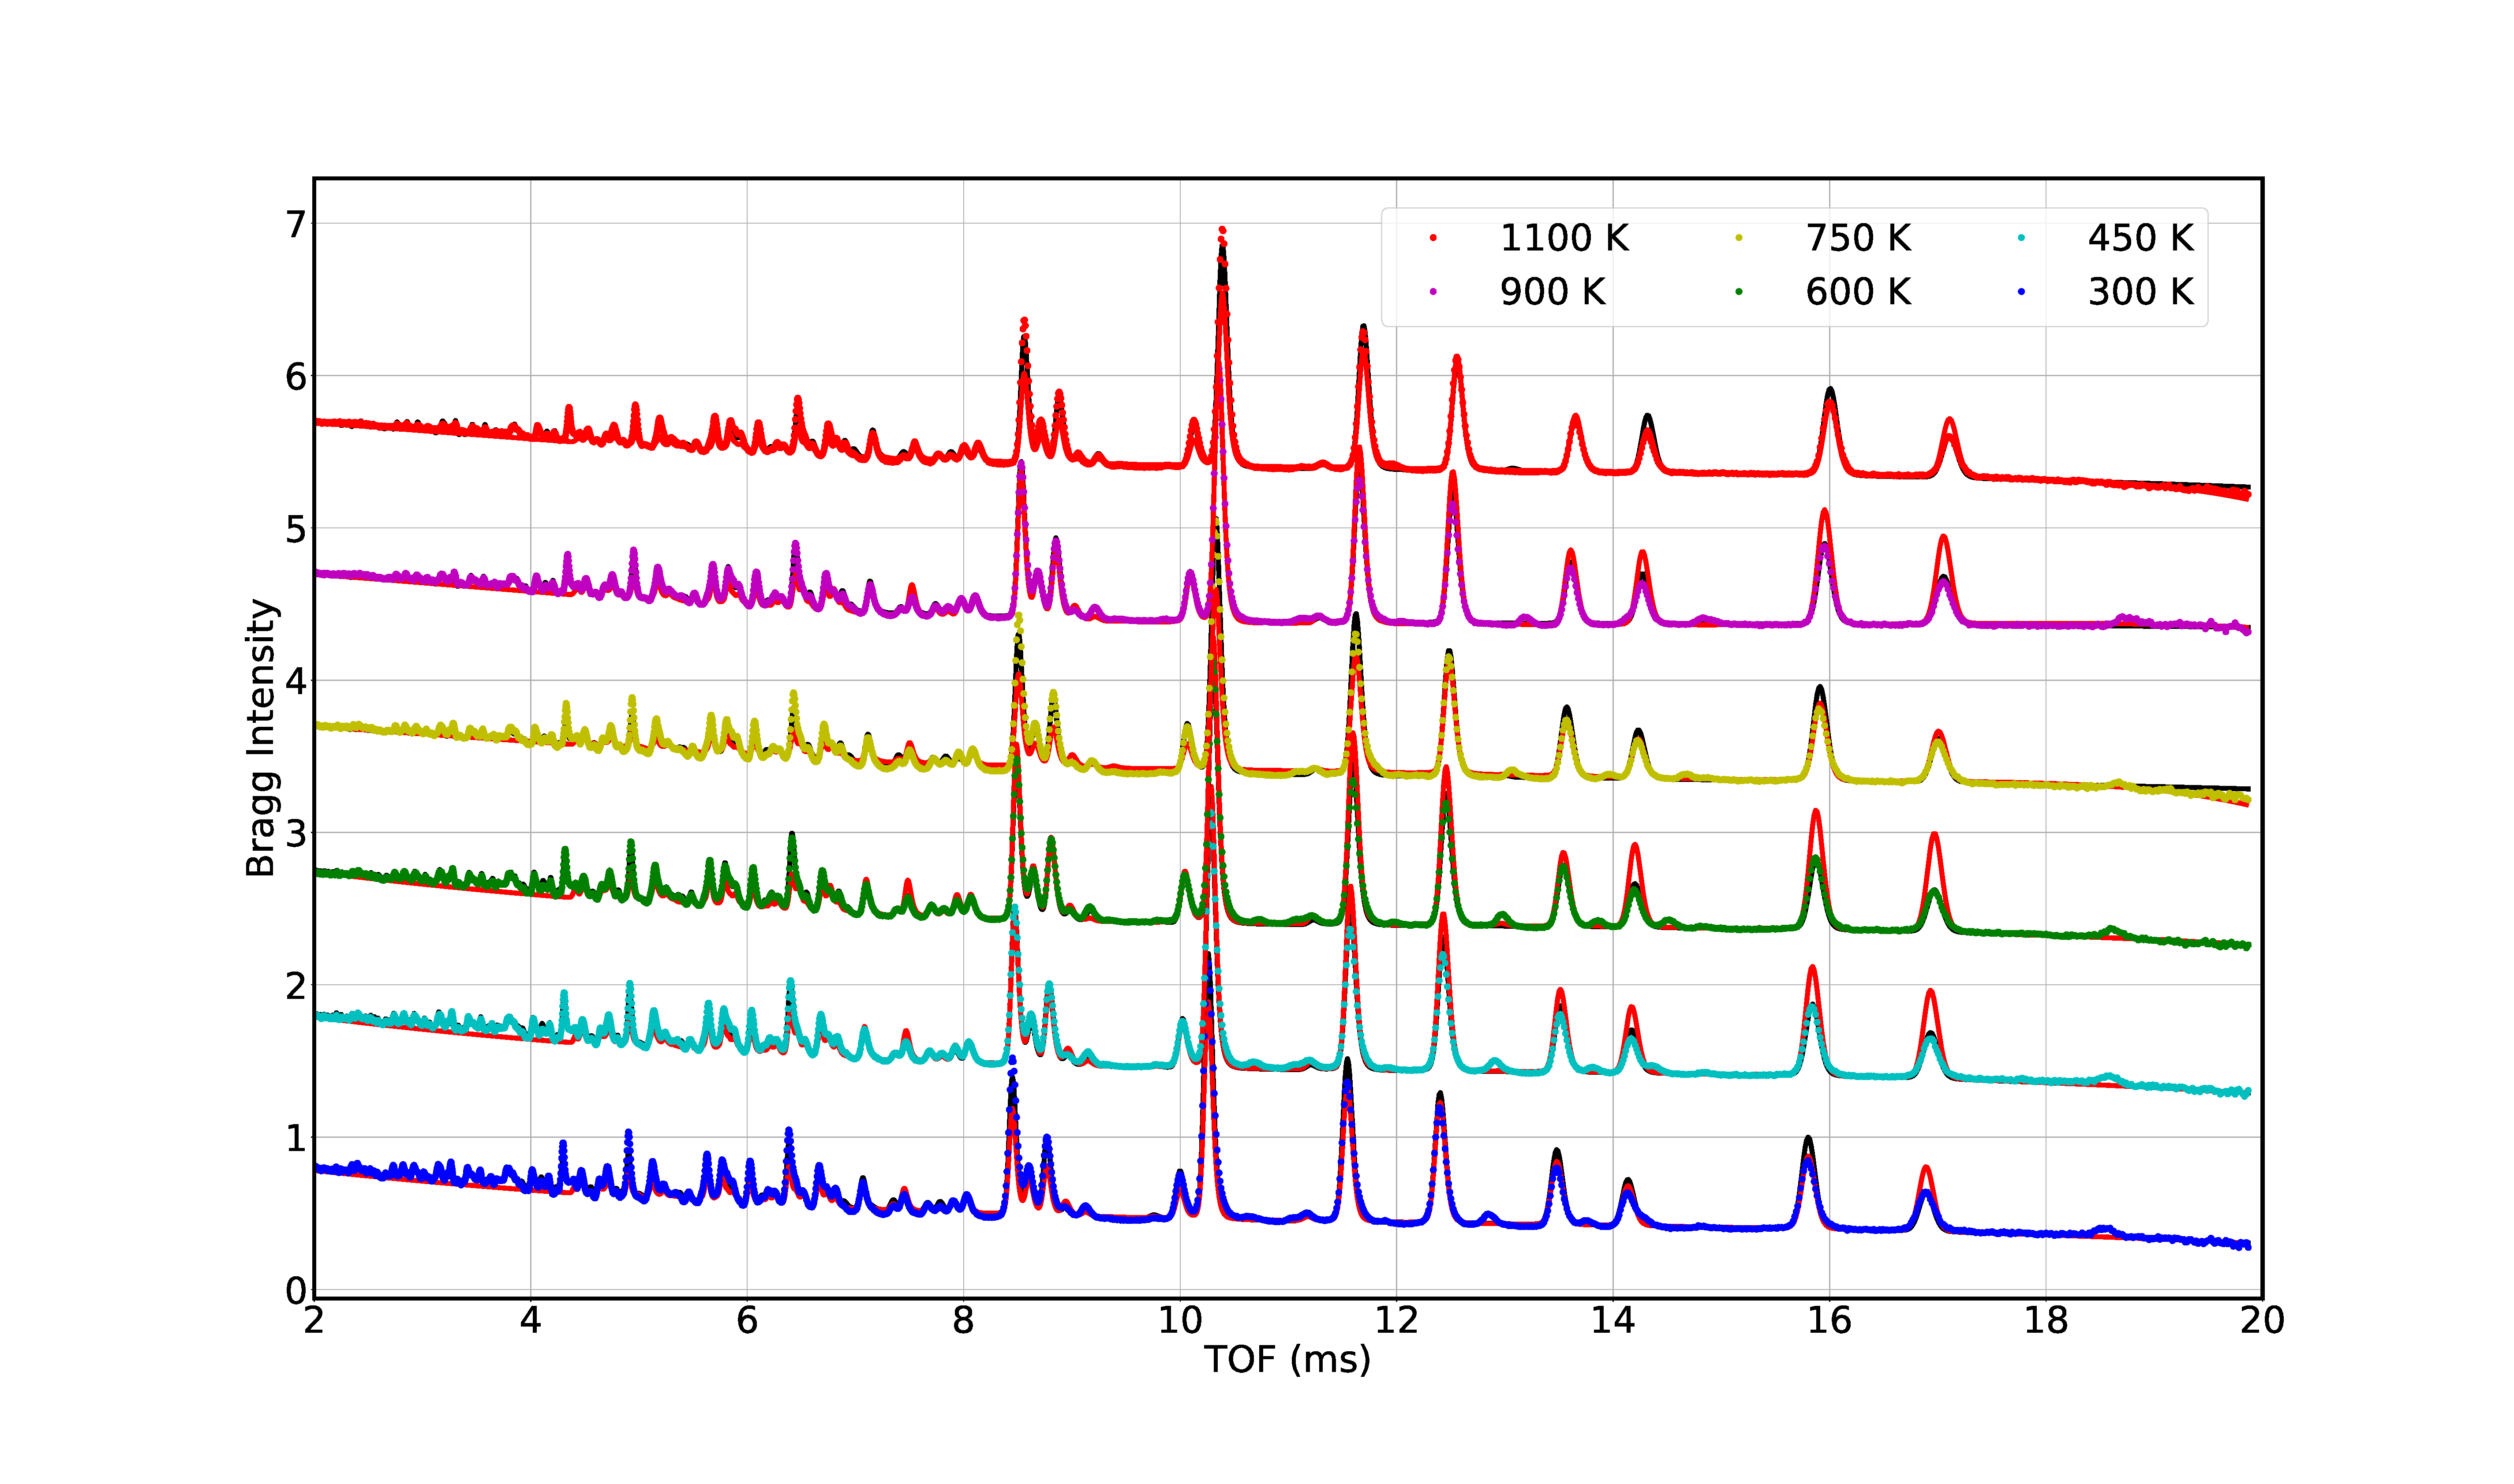
\includegraphics[width=0.5\textwidth]{Pics/bragg.pdf}
\caption{The Bragg diffraction data. The data are represented as circles with constant offset to separate those curves.
The solid black lines indicate the  calculated intensities from GSAS, and RMC modeling are represented by the solid red lines. }
\label{fig:Rietveld_refinement}
\end{figure}

\subsection{Local Structure Analysis}
The synchrotron pair distribution function $D(r)$ defined as functions \ref{fun:dofr_0} and \ref{fun:dofr_1}, are shown in Fig. \ref{fig:xpdf}.
The first peak corresponds to the La-O nearest-neighbor distance at around 2.5~\AA, and the second peaks refers to La-Zr around 3.6~\AA.
The position and integrated area are constant for all temperatures,
reflection there is no significant differences in crystal framwork structure. The higher-$r$ PDF shows shifting and broadening of the peaks as the temperature rising,
because of the increases of the lattice parameters.

 The RMC analysis used 4 data sets to perform RMC fits, including Bragg data (Fig.\ref{fig:Rietveld_refinement}) and PDF $D(r)$ from neutron total scattering (Fig.\ref{fig:npdf}),
 and scattering function $i(Q)$ from both neutron (Fig.\ref{fig:nsoq})  and synchrotron experiments(Fig.\ref{fig:xsoq}) .


The low-$r$  distributions of distances from the RMC and MD configurations are shown in Fig.\ref{fig:partialPDFwithLi} and  Fig.\ref{fig:partialPDFwithoutLi}. The interesting point about these diagrams is that
the Li-X (X represents Li, La, Zr or O) distribution from RMC are smoother than those from MD in all temperatures, as shown in Fig.\ref{fig:partialPDFwithLi}, indicating the Li-ion movement remains  disorderly.
But the framework structure keep stable in each case as shown in Fig.\ref{fig:partialPDFwithoutLi}, which is consist with the result of XPDF as shown in Fig. \ref{fig:xpdf}.




\begin{figure}[t]
\centering
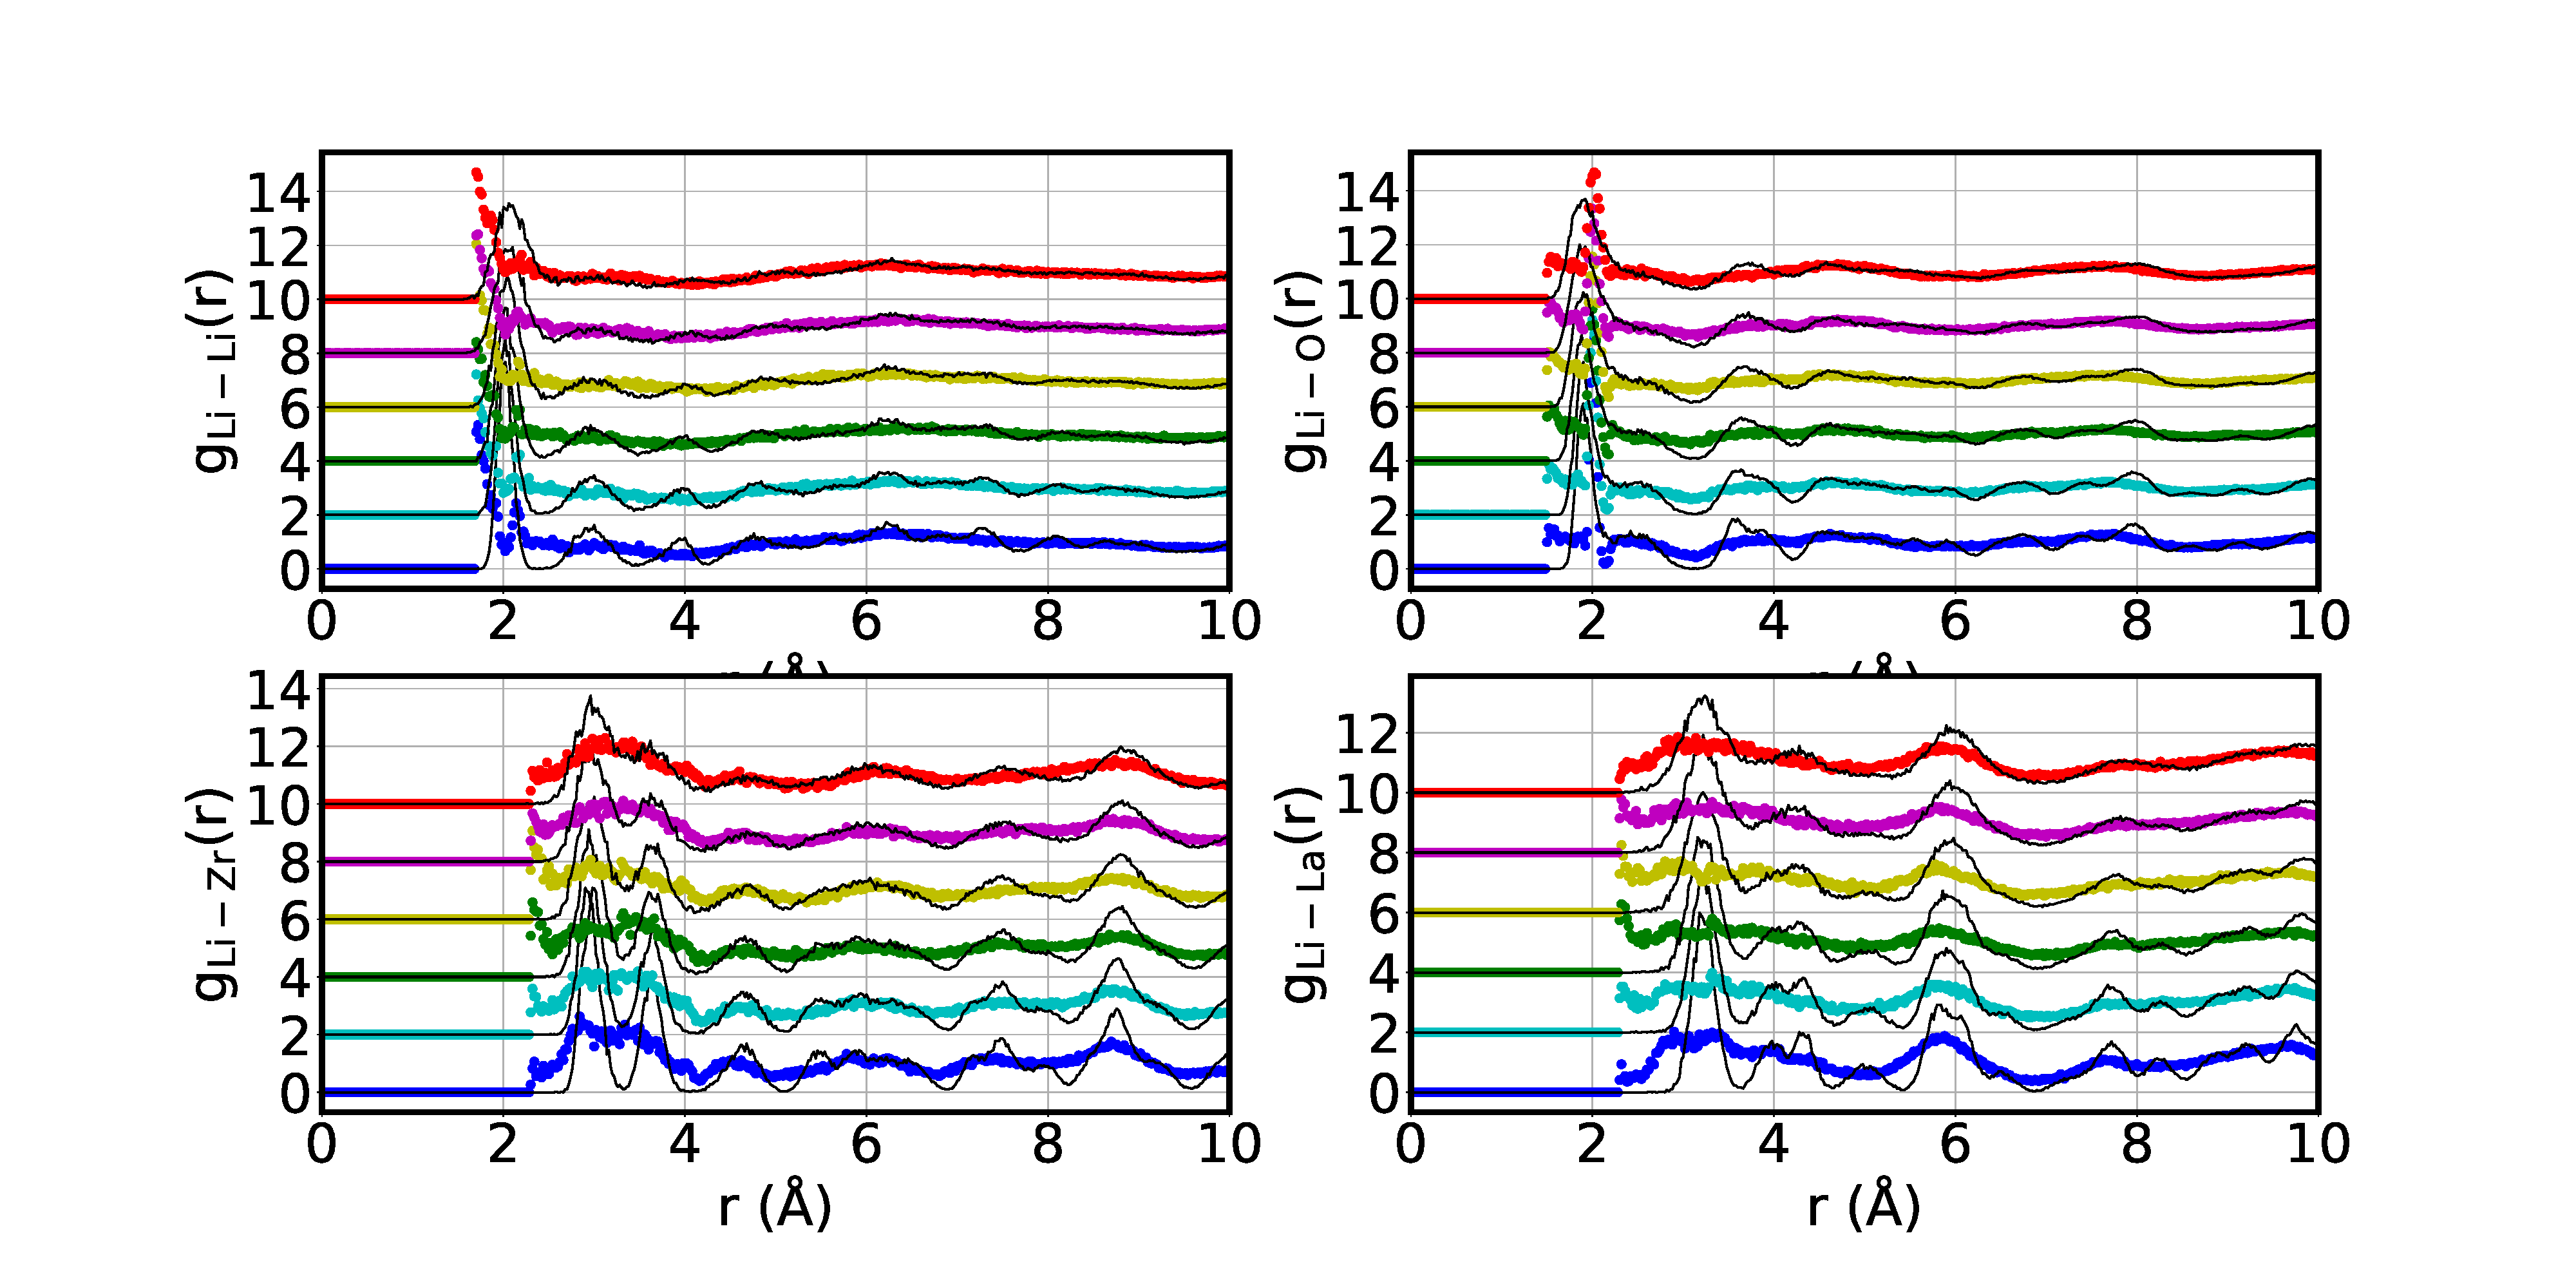
\includegraphics[width=0.5\textwidth]{Pics/partialPDFwithLi.pdf}
\caption{The distributions calculated from RMCProfile of (1) Li-Li, (2)Li-O, (3)Li-Zr, (4)Li-La at low-$r$ range for all temperatures. A constant offset has been applied to separate those curves.}
\label{fig:partialPDFwithLi}
\end{figure}

\begin{figure}[t]
\centering
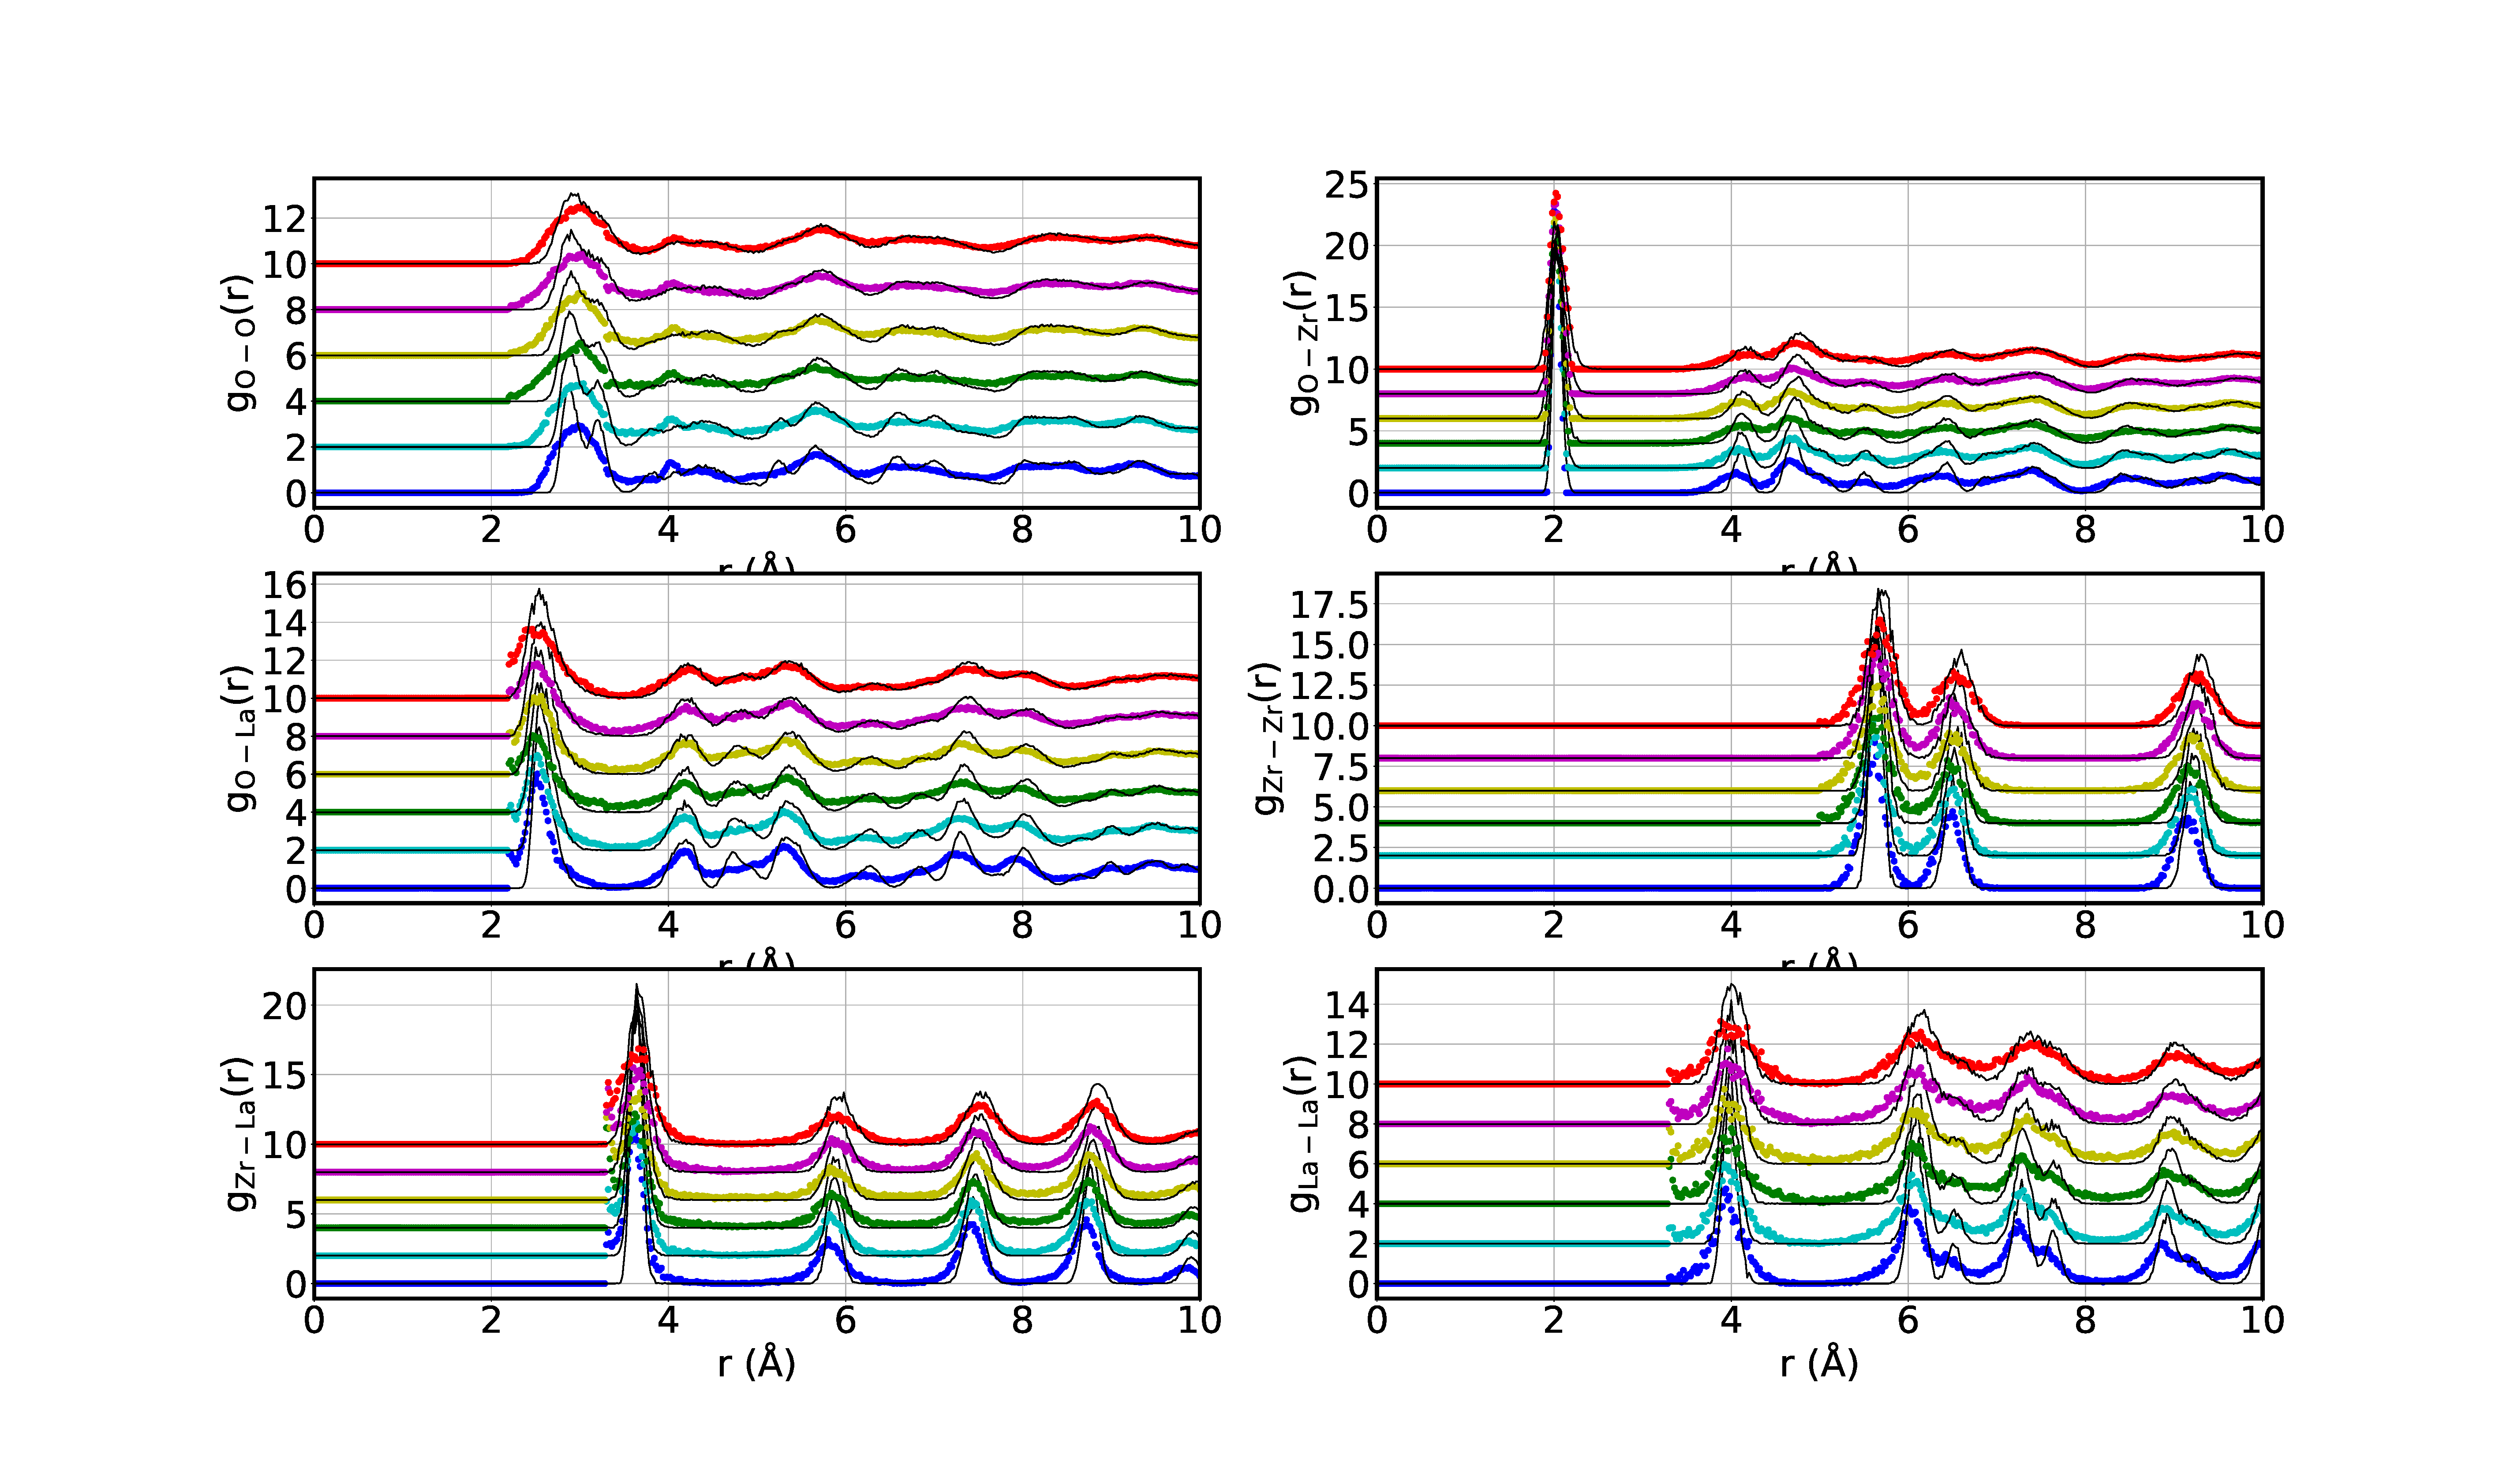
\includegraphics[width=0.5\textwidth]{Pics/partialPDFwithoutLi.pdf}
\caption{The distributions calculated from RMCProfile of (1) O-O;(2) O-Zr;(3) O-La; (4) Zr-Zr; (5) Zr-La; (6) La-La at low-$r$ range for all temperatures. A constant offset has been applied to separate those curves. The solid lines (black) indicate the values obtained from Molecular Dynamic simulation}
\label{fig:partialPDFwithoutLi}
\end{figure}


\subsection{Electrochemical Impedance Spectroscopy}

The EIS of the LLZO were examined with a in-plane geometry at elevated temperatures from -20$^\circ$C to 100$^\circ$C, as shown in  Fig.\ref{fig:impedance}.
From the Nyquist plots, a typical semi arc with the straight tail indicates the ion in-plane diffusion at low frequency occurs along the LLZO.
The ion conductivity is about 2.1$\times$10$^{-4}$ S/cm at room temperature.

\begin{figure}[t]
\centering
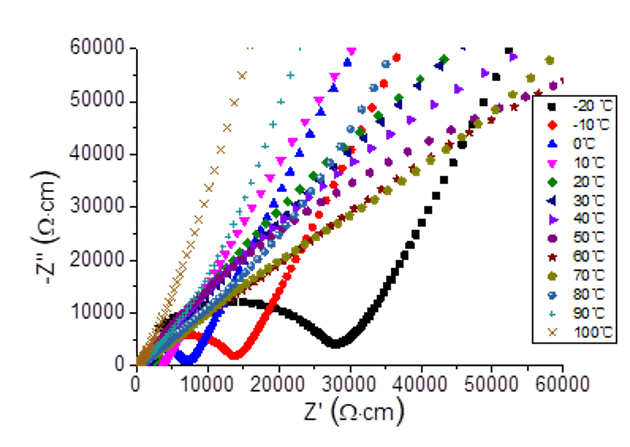
\includegraphics[width=0.5\textwidth]{Pics/impedance.png}
\caption{AC impedance data collected from -20$^\circ$C to 100$^\circ$C.}
\label{fig:impedance}
\end{figure}

The activation energy can be calculated from the series of EIS at elevated temperatures shown in Fig.\ref{fig:arrhenius-plot}.
The activation energy E$_a$ is estimated based on the Arrhenius equation for the ionic conductivity

\begin{equation}
\sigma T = \sigma_0 e^{-E_a/k_B T}
\end{equation}


\begin{figure}[t]
\centering

\includegraphics[width=0.5\textwidth]{Pics/arrhenius-plot.png}
\caption{A plot of conductivity as a function of temperature for LLZO. The line indicates an Arrhenius fit over the whole temperature range.}
\label{fig:arrhenius-plot}
\end{figure}

where $\sigma$ is the ionic conductivity, $\sigma_0$ is a pre-exponential factor, T is the absolute temperature, and k$_B$ is the Boltzmann constant.
Furthermore, the diffusion coefficient was calculated using the Nernst-Einstein-equation

\begin{equation}
D=\frac{\sigma k_B T}{N_{Li} q^2}
\end{equation}

where q is the charge of the lithium and N$_{Li}$ the concentration of lithium, in this case for a cubic LLZO structure.
The calculated activation energy is about 0.36~eV which is in good agreement to other publications,
as well as the diffusion coefficient shown in Fig.\ref{fig:DiffusionCoefficient} with 1.31 $\times$ 10$^{-13}$ m$^2$s$^{-1}$ at room temperature.



\begin{figure}[t]
\centering
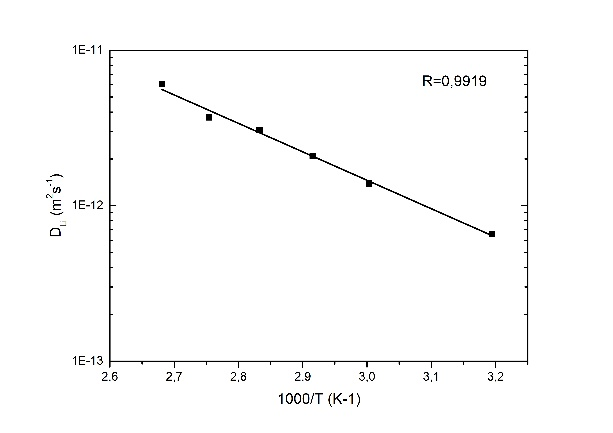
\includegraphics[width=0.5\textwidth]{Pics/DiffusionCoefficient.png}
\caption{Diffusion coefficient at different temperatures}
\label{fig:DiffusionCoefficient}
\end{figure}


\subsection{Lithium Distribution and Dynamics Analysis}



The 3D density maps of Li in cubic garnets are shown in Fig.\ref{fig:pdfs}.
The lithium distribution can ben expected in liquid and amorphous materials

\begin{figure*}[t]
\centering
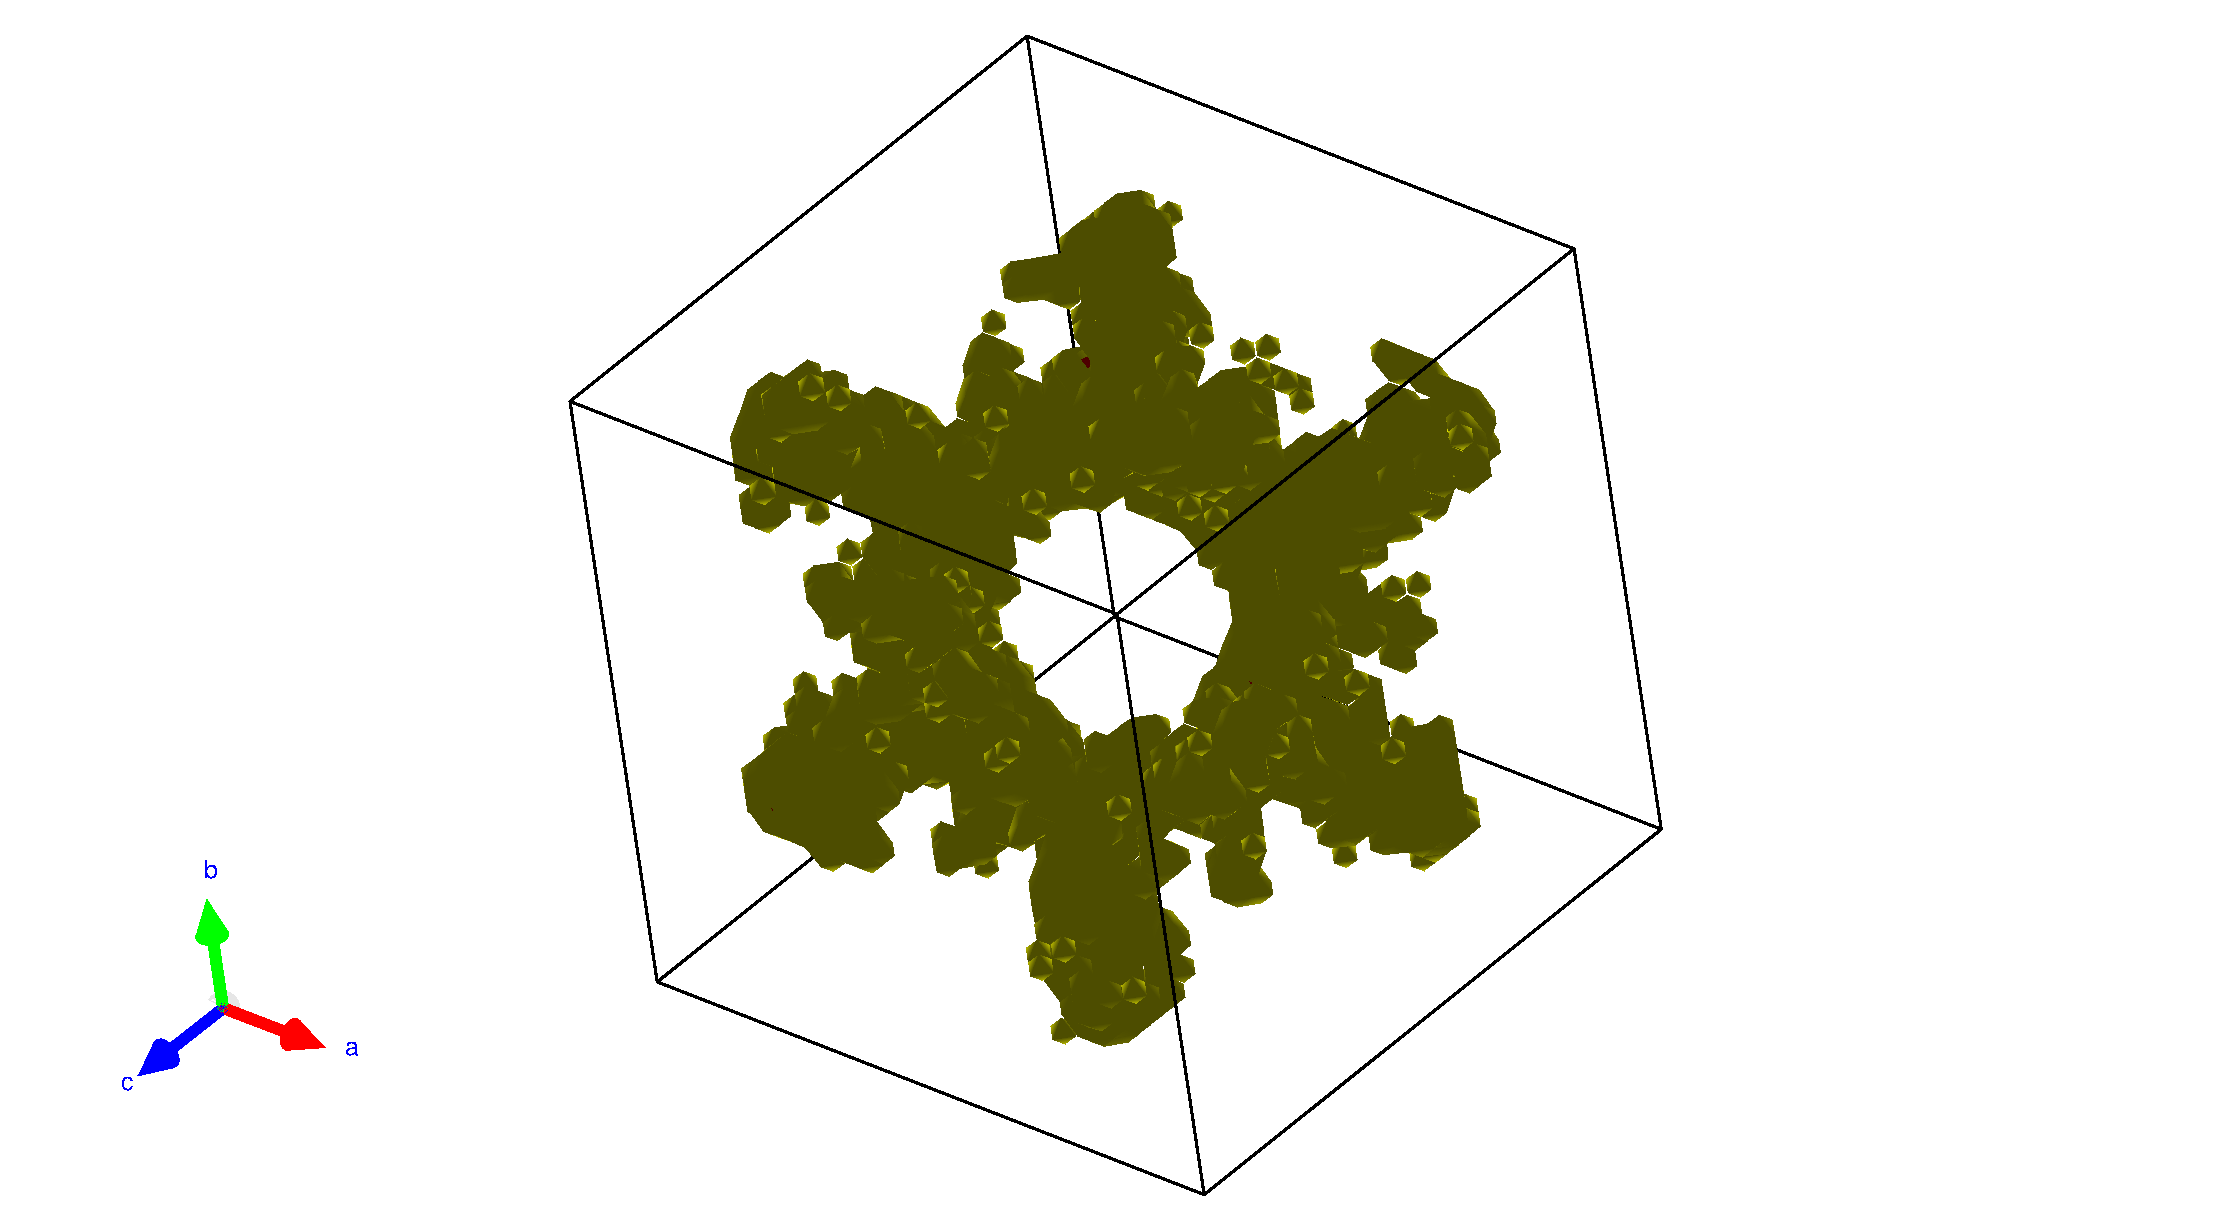
\includegraphics[width=0.9\textwidth]{Pics/pdfs.pdf}
\caption{Isosurfaces with level of 0.1~\AA$^{-3}$ (yellow) and 3~\AA$^{-3}$ (red)}
\label{fig:pdfs}
\end{figure*}

\begin{figure}[t]
\centering
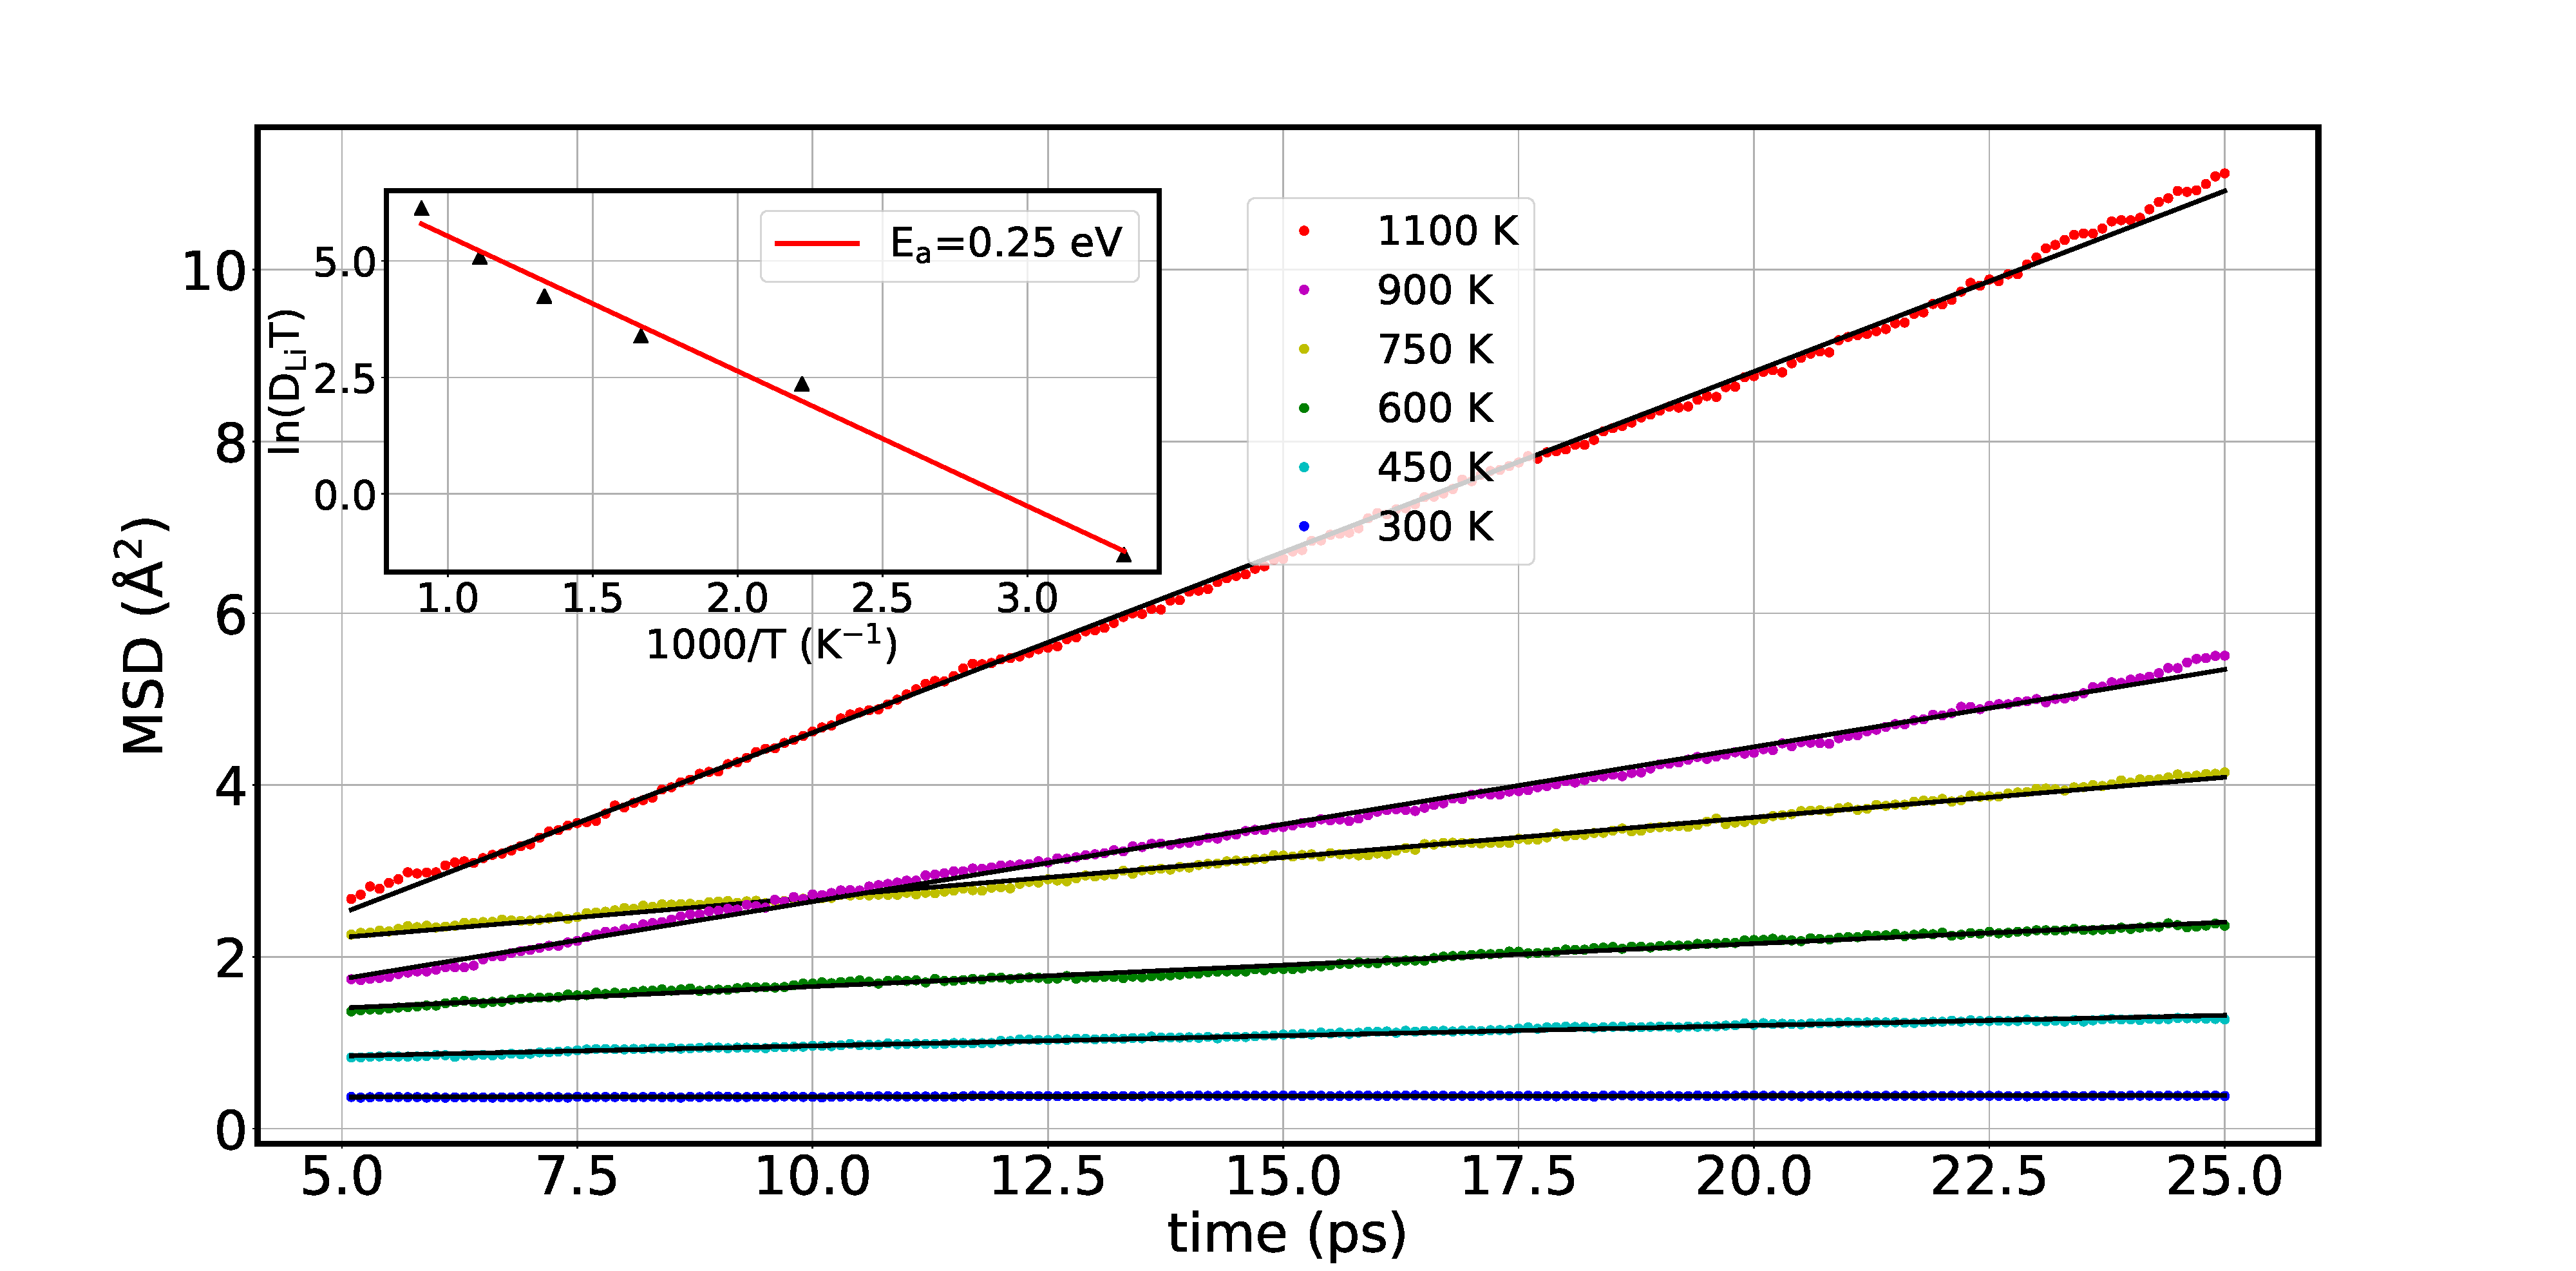
\includegraphics[width=0.5\textwidth]{Pics/MSD.pdf}
\caption{Mean squared displacement (MSD) of Li from 300 K to 1100 K.
The slope of MSD of each temperature data set yields the diffusion constant (D).
The inset shows a diffusion constant (D) versus temperatures.}
\label{fig:msd}
\end{figure}


%\begin{figure}
%\centering
%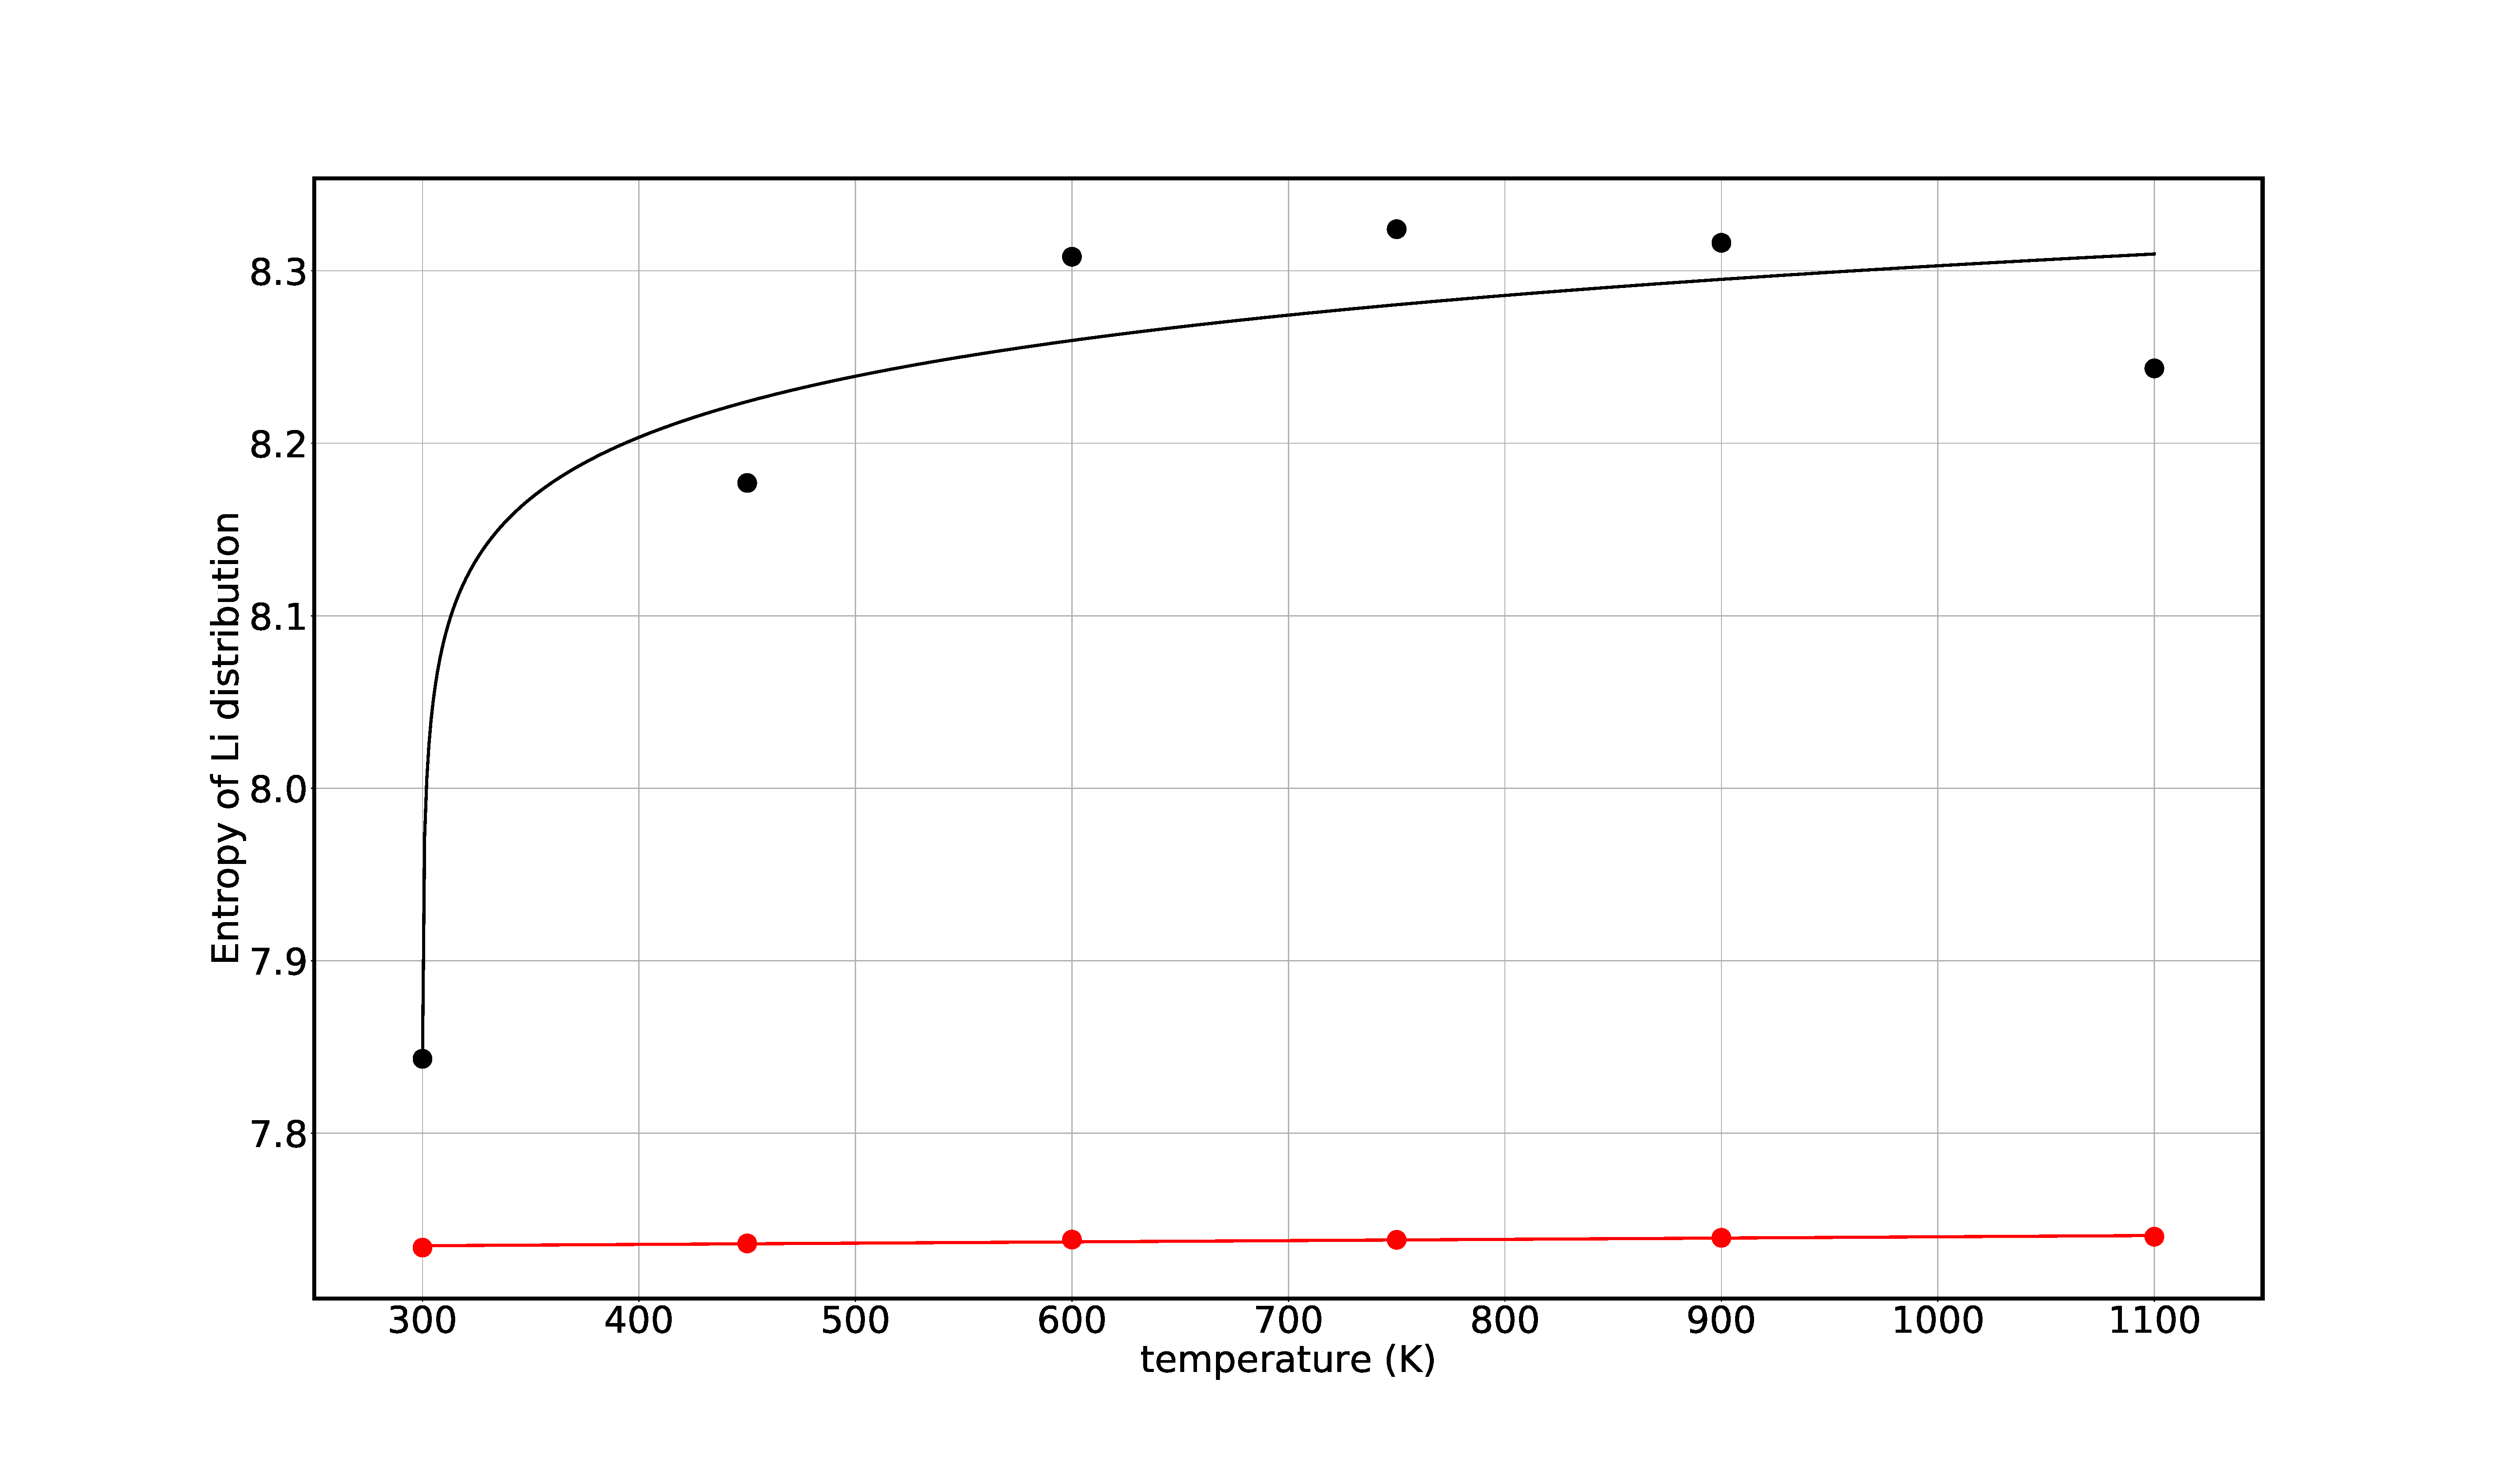
\includegraphics[width=0.5\textwidth]{Pics/entropy.pdf}
%\caption{The entropy of Li distribution. Data represented by back circles are the experimentally determined values using RMC refinement.
%Red circles represent the Molecular Dynamic simulation ones.}
%\label{fig:entropy}
%\end{figure}


%\begin{figure}
%\centering
%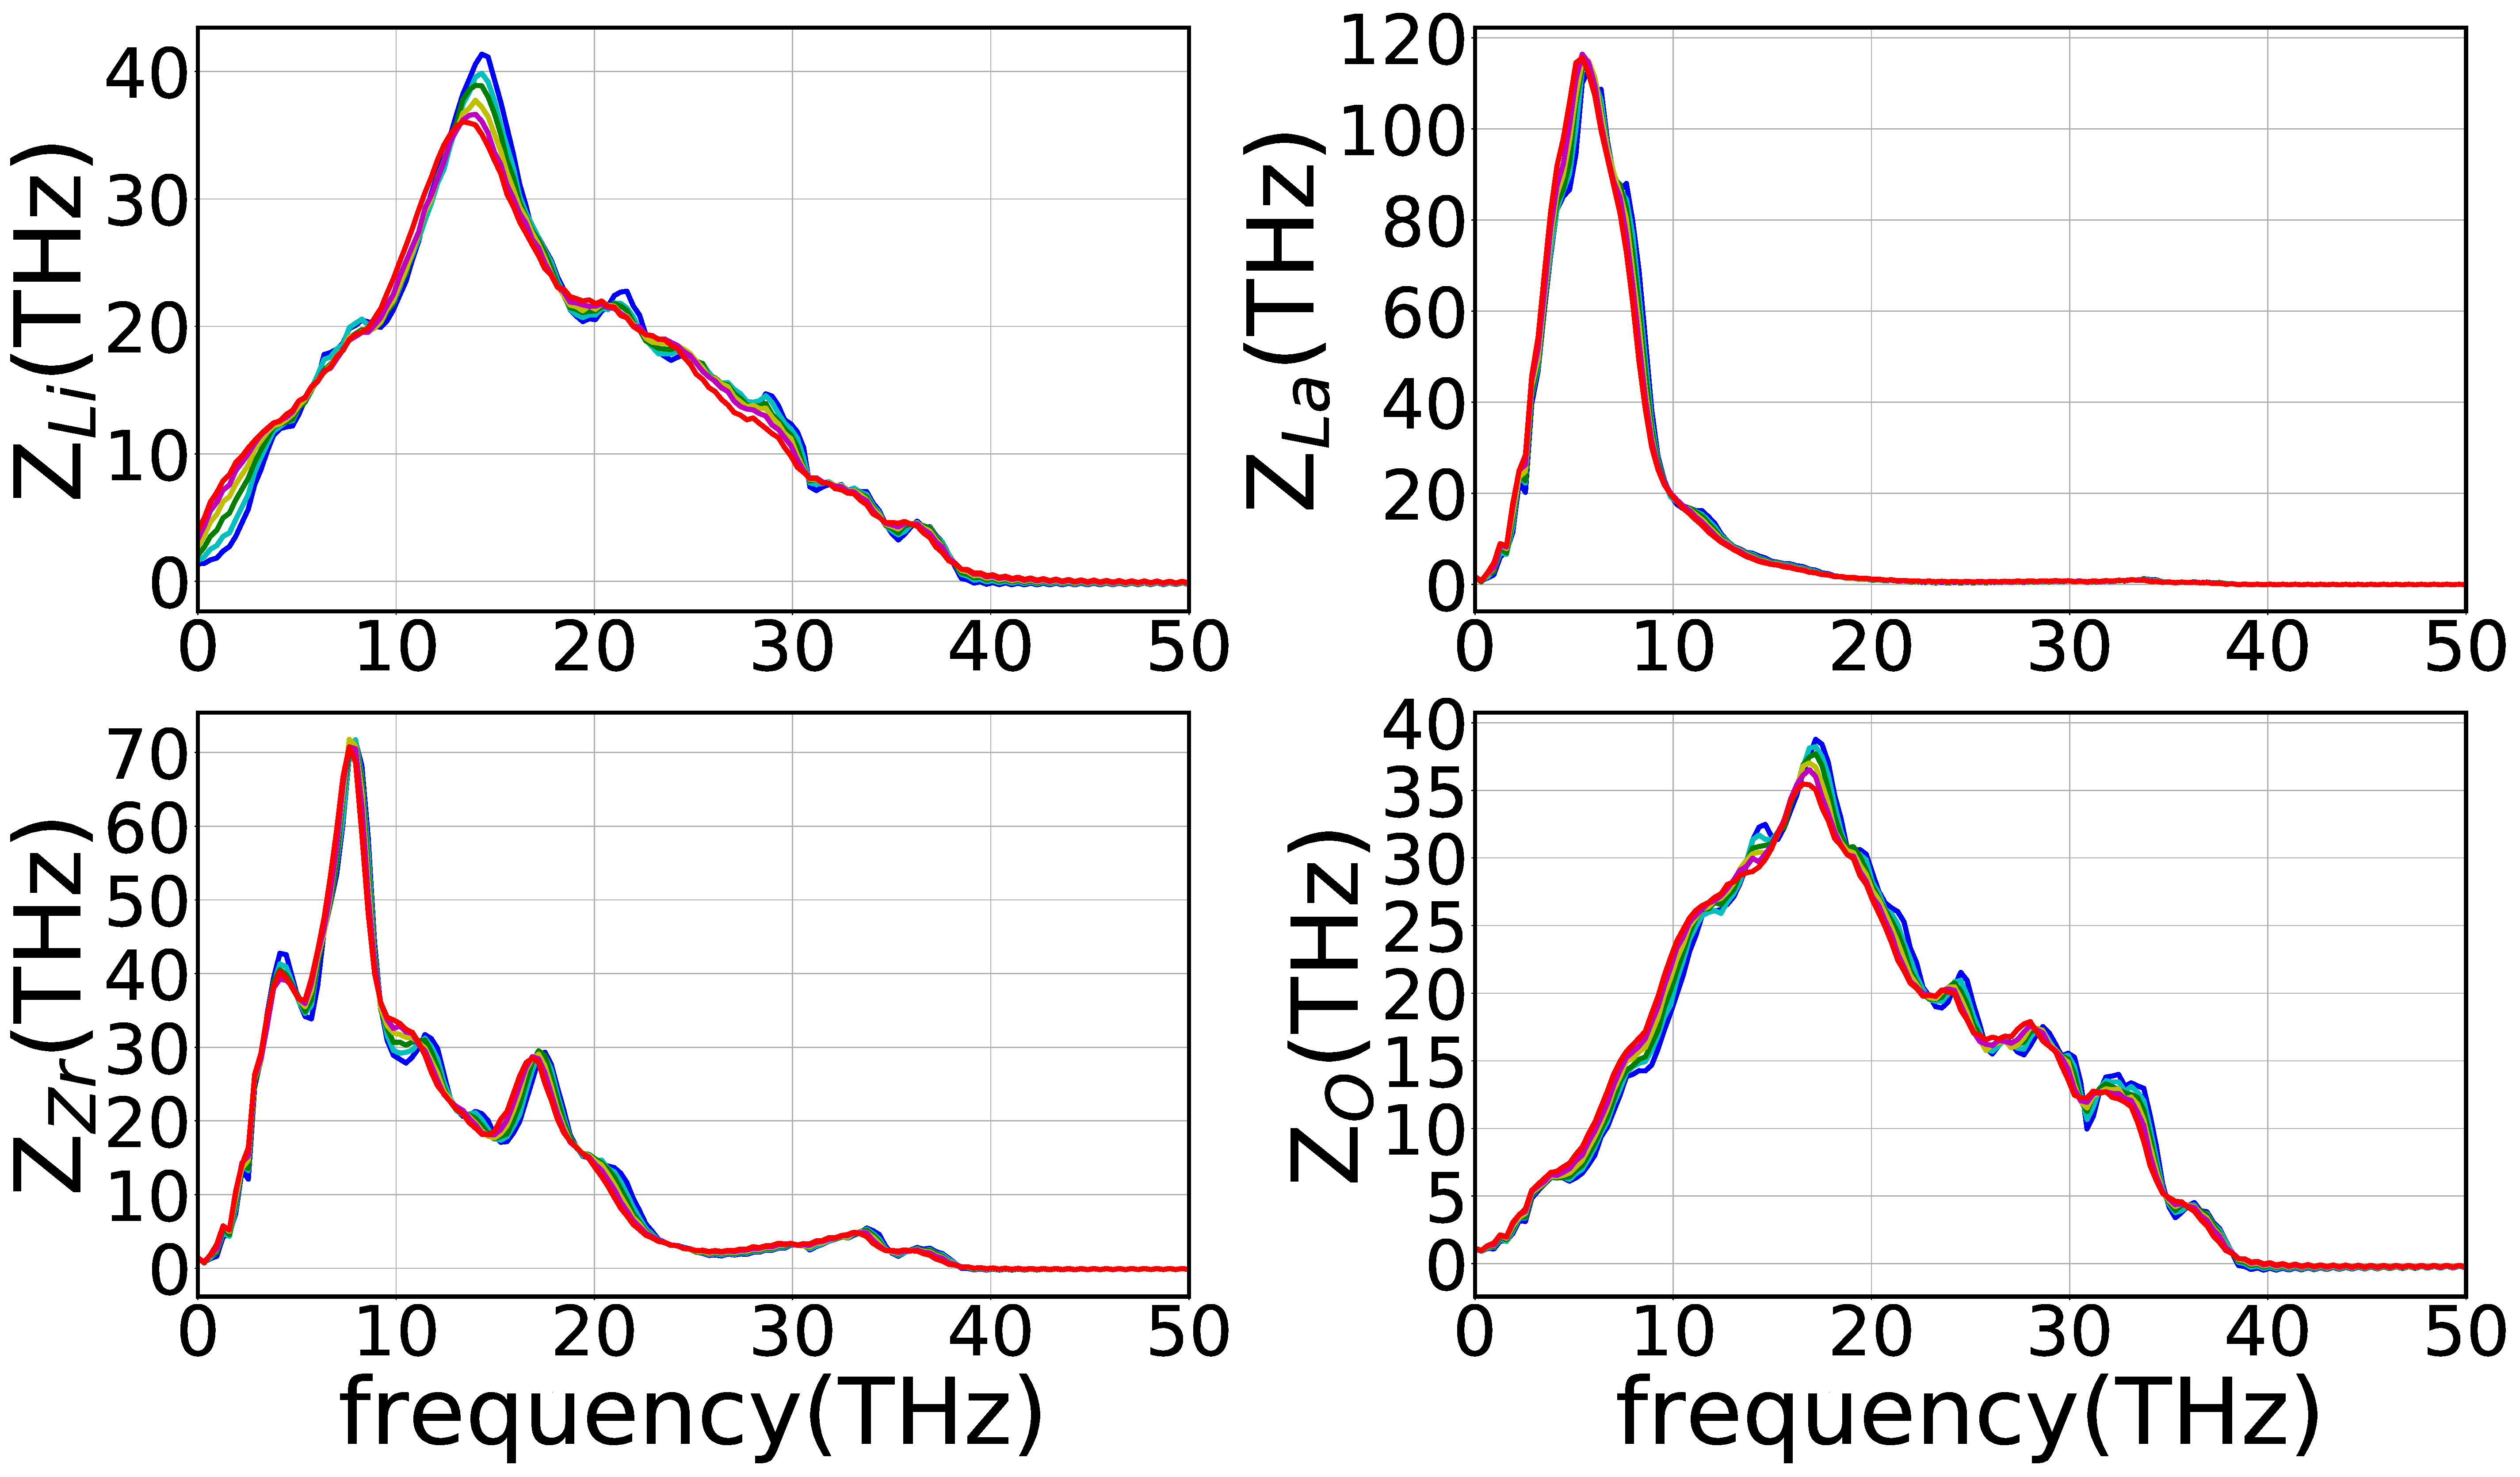
\includegraphics[width=0.5\textwidth]{Pics/powerSpectra.pdf}
%\caption{The power spectrum of Li vibrational frequencies.
% The zero point of power spectrum for each temperature yields the diffusion constant.
% The inset shows a diffusion constant (D) versus temperatures.}
%\label{fig:powerSpectra}
%\end{figure}


%\section{Simple model}\label{sec:model}
%
%\subsection{Description of the simple model}
%
%We have constructed a very simple model of the octahedral network, with sufficient interaction terms to reproduce the essential dynamics but few enough to give control of how the will behave. We consider composition AX$_3$, with corner-linked AX$_6$ octahedra. The first term is a Morse function to describe the change in separation $r$ of nearest-neighbour A--X bonds:
%\begin{equation}
%\label{eq:bond}
%E(r) = D \left[ \exp\left( - 2 \alpha (r - r_o) \right) - 2 \exp\left( - \alpha (r - r_o) \right) \right]
%\end{equation}
%This function has the advantage over a simple harmonic interaction that because it has anharmonicity it will give some thermal expansion of the A--X bond. Although there are three parameters, the zero-temperature distance $r_0$ simple sets a length scale. Given that we are not interested in the dissociation energy $D$ per se,
%the second differential evaluated at equilibrium, $E^{\prime \prime}_0 = 2 \alpha^2 D$, gives as the stretching frequency of the A--X bond and thus in practice we only need consider one parameter to be of interest. The parameter $D$ can be tuned to give the highest calculated vibrational frequency to be consistent with experimental measurements or ab initio calculations.
%
%The other two function concerns the bond angles. For the X--A--X angle of equilibrium value $90^\circ$, $\theta$, we use a potential energy function of the form
%\begin{equation}
%\label{eq:rightangle}
%E(\theta) = \tfrac{1}{2} k  \cos^2 \theta
%\end{equation}
%where $k$ is the force constant. For the linear A--X--A bond angle, $\phi$, we use a function of the form
%\begin{equation}
%E(\phi) = A (1 +  \cos \phi)
%\label{eq:linearangle}
%\end{equation}
%where $A$ is the force constant. This latter function has higher stability around $\phi = 180^\circ$. The value of the parameter $A$ give a non-zero frequency to the rigid unit modes. In principle $A$ could have negative values, which would cause a phase transition to a distorted state but one without complete order because all RUM distortions can condense simultaneously. The parameter $k$ controls the stiffness of the AX$_6$ octahedra. In the limit $k = 0$ we have a system of rigid bonds.
%
%Starting values of the force constants $D$, $\alpha$, $k$ and $A$ were estimated by calculating the phonon dispersion curves for ScF$_3$ with appropriate masses, and comparing with those calculated by DFT. Calculations were performed using the GULP code \cite{Gale:2003eo,Gale:1997iq}.  The value of $r_0 = 2.0125$~\AA\ was set as half the unit cell length of ScF$_3$, the value of $\alpha$ was arbitrarily set as 1.55~\AA$^{-1}$, The value of $D$ was set as 2.0~eV to math the highest frequency with that of ScF$_3$, the value of $A$ was set as 0.025~eV to give the rotational phonon frequency for wave vectors between the points M and R to be similar to that of ScF$_3$, and the value of $k$ was set as 1.5~eV to ensure that a matching of the frequencies of the transverse acoustic modes, which give rise to bending of the corresponding bond angle. The calculated dispersion curves are shown in Figure \ref{fig:dispersioncurves}. In this diagram we colour the dispersion curves according to the value of the mode Gr\"{u}neisen parameter following methods we have described previously \cite{Rimmer:2015km}. What is interesting is the extent to which the simple model reflects the DFT dispersion curves, both in overall shape and in the distribution of values, including sign, of mode Gr\"{u}neisen parameters. The main peculiarity of the model is that the elastic constant $C_{12} = 0$, far from the normal Cauchy relationship for cubic materials with central forces of $C_{12} = C_{44}$. This has little effect on the physical properties.
%
%\begin{figure}[t]
%\begin{center}
%\includegraphics[width=0.4\textwidth]{dispersion_curves.pdf}
%\caption{Calculated dispersion curves of ScF$_3$ based on the model indicated in equations \ref{eq:bond}--\ref{eq:linearangle}. The curves are coloured red or blue depending on the sign of the mode Gr\"{u}neisen parameter, as discussed in the text, with the intensity of the colour reflecting the size of the mode Gr\"{u}neisen parameter up to some saturation value. In this calculation $D = 2.0$~eV, $r_0 = 2.0125$~\AA, $\alpha = 1.55$~\AA$^{-1}$, $k = 1.5$~eV, and $A = 0.025$~eV.}
%\label{fig:dispersioncurves}
%\end{center}
%\end{figure}
%
%In principle this model contains all the essential interactions to give negative thermal expansion, a characteristic of ScF$_3$ and ReO$_3$ if not of many other perovskites other than when associated with a displacive phase transition or through magnetic/electronic effects.



\section{Conclusions}
The conclusions section should come in this section at the end of the article, before the Conflicts of interest statement.

\section{Appendix}

\subsection{The Correlation Functions}

Time-dependent correlation functions are valuable tools to describe the average way the quantity will change with time,
and predict the trends within the behaviour of atomic structure and dynamics.


One of the simplest correlation function for velocity with a mean value of zero, $C(t)$, is defined as
%x
 \begin{equation}
C(t)=\frac{\langle v(0)v(t)\rangle}{\langle | v(0)|^2 \rangle}
=\frac{(\lim \mathcal{T}\rightarrow \infty) \frac{1}{\mathcal{T}} \int^{\mathcal{T}}_{0} v(t')v(t+t')dt' }{\langle v^2 \rangle}
\end{equation}

For  the harmonic crystal, the velocity of the $j$-th atom is given as

\begin{equation}
v_j(t)=\frac{-i}{(Nm_j)^{1/2}}\sum_{\textbf{k},v}\omega(\textbf{k},v)\textbf{e}_j(\textbf{k},v)exp(i\textbf{k}\cdot \textbf{r})Q(\textbf{k},v,t)
\end{equation}

and leads to the classical result:
\begin{equation}
\sum_j  m_j \langle |v_j(t)\cdot v_j(0) |\rangle = \frac{k_B T}{N}\sum_{\textbf{K},v}\cos (\omega(\textbf{k}, v)t)
\end{equation}

In addition, the power spectra $Z(\omega)$ is given by the Fourier transform of $C(t)$:

\begin{equation}
Z(\omega)=\int C(t)exp(-i\omega t)dt
\end{equation}

It can be seen that the power spectrum of the mass-weighted velocity correlation function is equal to the phonon density of states.

Consider another correlation function for position of atom, $G_s(r,t)$, is defined as

\begin{align*}
G_s(\Delta r,t)&=\frac{\langle r(0)r(t)\rangle}{\langle | r(0)|^2 \rangle} \\
        &=\frac{1}{N}\sum_{j}^{N}\int \langle \delta(r'-r_j(0))\delta(r'+\Delta r -r_j(t))dr' \rangle \\
        &=\frac{1}{N}\langle \sum_{j}^{N}\delta(\Delta r +r_j(0)-r_j(t))\rangle
\end{align*}

which is related to the probability of finding an atom in the volume $dr$ at position $\Delta r$ for a time interval of $t$,
and can be named as self-part of van Hove correlation function.

The mean square displacement (MSD) $\langle \Delta r_i(t)\rangle ^2$  is a measure of the deviation of the position of an atom with
respect to a reference position over time. MSD is related to the $G_s(r,t)$ as:

\begin{equation}
  \langle \Delta r_i(t)\rangle ^2=\int_{0}^{\infty} (\Delta r_i(t))^2\cdot 4\pi(\Delta r_i(t))^2G_s(\Delta r,t)d\Delta r
\end{equation}

\subsection{ Nernst-Einstein  Equation}

The value of ionic conductivity ($\sigma$) is determined by the impedance spectroscopy.
In solid electrolytes, as the anions are immobile, the ionic conduction is driven by the diffusion of Li$^+$ ions.
The connection between the diffusion constant (D) and $\sigma$ is defined by the Nernst-Einstein (NE) equation,
which are widely used for electrolyte system. NE equation is given as

\begin{equation}
D(T)=\frac{kT}{Ne^2}\sigma(T)
\end{equation}

where $k$ is the Boltzmann constant, $e$ is the elementary charge, and N is the number of carrier ions.

\section*{Conflicts of interest}
There are no conflicts to declare.

\section*{Acknowledgements}
The Acknowledgements come at the end of an article after Conflicts of interest and before the Notes and references.

%%%END OF MAIN TEXT%%%

%The \balance command can be used to balance the columns on the final page if desired. It should be placed anywhere within the first column of the last page.

\balance

%If notes are included in your references you can change the title from 'References' to 'Notes and references' using the following command:
%\renewcommand\refname{Notes and references}

%%%REFERENCES%%%
\bibliography{rsc} %You need to replace "rsc" on this line with the name of your .bib file
\bibliographystyle{rsc} %the RSC's .bst file

\end{document}
